\chapter{CMB Morphology and Topology}\label{ch:T3}

\providecommand{\TaNsimMF}{}\renewcommand{\TaNsimMF}{300}
\providecommand{\TaPatchDeg}{}\renewcommand{\TaPatchDeg}{12.8}
\providecommand{\TaPixArcmin}{}\renewcommand{\TaPixArcmin}{1.5}
\providecommand{\TaSigZero}{}\renewcommand{\TaSigZero}{93.8}
\providecommand{\TaSigZeroSky}{}\renewcommand{\TaSigZeroSky}{104.2}
\providecommand{\TaThetaC}{}\renewcommand{\TaThetaC}{12.0}
\providecommand{\TaThetaCSky}{}\renewcommand{\TaThetaCSky}{13.4}
\providecommand{\TaVzeroOne}{}\renewcommand{\TaVzeroOne}{0.1587}
\providecommand{\TaVzeroOneSim}{}\renewcommand{\TaVzeroOneSim}{0.1585}
\providecommand{\TaChiDevPct}{}\renewcommand{\TaChiDevPct}{1.4}
\providecommand{\TaChiErrPct}{}\renewcommand{\TaChiErrPct}{0.8}
\providecommand{\TaChiPeakPatch}{}\renewcommand{\TaChiPeakPatch}{78}
\providecommand{\TaChiOne}{}\renewcommand{\TaChiOne}{73}
\providecommand{\TaChiMinusOne}{}\renewcommand{\TaChiMinusOne}{-84}
\providecommand{\TaEulerOurs}{}\renewcommand{\TaEulerOurs}{89}
\providecommand{\TaEulerSkimage}{}\renewcommand{\TaEulerSkimage}{89}
\providecommand{\TaHotSpotsSky}{}\renewcommand{\TaHotSpotsSky}{7157}
\providecommand{\TaPatchArea}{}\renewcommand{\TaPatchArea}{164}
\providecommand{\TbNsim}{}\renewcommand{\TbNsim}{300}
\providecommand{\TbA}{}\renewcommand{\TbA}{0.05}
\providecommand{\TbB}{}\renewcommand{\TbB}{0.1}
\providecommand{\TbSixA}{}\renewcommand{\TbSixA}{0.30}
\providecommand{\TbLocSzero}{}\renewcommand{\TbLocSzero}{0.298}
\providecommand{\TbLocSone}{}\renewcommand{\TbLocSone}{0.300}
\providecommand{\TbLocStwo}{}\renewcommand{\TbLocStwo}{0.299}
\providecommand{\TbNlSzero}{}\renewcommand{\TbNlSzero}{0.493}
\providecommand{\TbNlSone}{}\renewcommand{\TbNlSone}{0.443}
\providecommand{\TbNlStwo}{}\renewcommand{\TbNlStwo}{0.470}
\providecommand{\TbLocMaxShiftPct}{}\renewcommand{\TbLocMaxShiftPct}{12}
\providecommand{\TbLocAreaMaxPct}{}\renewcommand{\TbLocAreaMaxPct}{0.0}
\providecommand{\TbNlAreaMaxPct}{}\renewcommand{\TbNlAreaMaxPct}{6.0}
\providecommand{\TbErrPct}{}\renewcommand{\TbErrPct}{1.0}
\providecommand{\TbNlResNu}{}\renewcommand{\TbNlResNu}{-2.0}
\providecommand{\TbNlResPct}{}\renewcommand{\TbNlResPct}{-1.9}
\providecommand{\TbNlResSig}{}\renewcommand{\TbNlResSig}{2.8}
\providecommand{\TcPatchCount}{}\renewcommand{\TcPatchCount}{76}
\providecommand{\TcPatchPlus}{}\renewcommand{\TcPatchPlus}{38}
\providecommand{\TcPatchMinus}{}\renewcommand{\TcPatchMinus}{38}
\providecommand{\TcNsim}{}\renewcommand{\TcNsim}{200}
\providecommand{\TcPred}{}\renewcommand{\TcPred}{1510}
\providecommand{\TcMean}{}\renewcommand{\TcMean}{1501}
\providecommand{\TcSd}{}\renewcommand{\TcSd}{39}
\providecommand{\TcSdPoisson}{}\renewcommand{\TcSdPoisson}{39}
\providecommand{\TcSdErr}{}\renewcommand{\TcSdErr}{2}
\providecommand{\TcMeanDevPct}{}\renewcommand{\TcMeanDevPct}{-0.6}
\providecommand{\TcMeanDevSig}{}\renewcommand{\TcMeanDevSig}{3.0}
\providecommand{\TcNetMax}{}\renewcommand{\TcNetMax}{0}
\providecommand{\TcPerDeg}{}\renewcommand{\TcPerDeg}{9.2}
\providecommand{\TcSame}{}\renewcommand{\TcSame}{17.3}
\providecommand{\TcOpp}{}\renewcommand{\TcOpp}{10.6}
\providecommand{\TcPoisson}{}\renewcommand{\TcPoisson}{14.0}
\providecommand{\TcSkyHundred}{}\renewcommand{\TcSkyHundred}{5310}
\providecommand{\TcSkyFiveHundred}{}\renewcommand{\TcSkyFiveHundred}{133315}
\providecommand{\TcSkyFiveHundredPatch}{}\renewcommand{\TcSkyFiveHundredPatch}{133453}
\providecommand{\TdNreal}{}\renewcommand{\TdNreal}{20}
\providecommand{\TdPixArcmin}{}\renewcommand{\TdPixArcmin}{0.59}
\providecommand{\TdFwhm}{}\renewcommand{\TdFwhm}{5}
\providecommand{\TdDefl}{}\renewcommand{\TdDefl}{1.81}
\providecommand{\TdKappa}{}\renewcommand{\TdKappa}{0.071}
\providecommand{\TdDetMin}{}\renewcommand{\TdDetMin}{0.38}
\providecommand{\TdMatchPct}{}\renewcommand{\TdMatchPct}{99.8}
\providecommand{\TdMatchMinPct}{}\renewcommand{\TdMatchMinPct}{99.6}
\providecommand{\TdSingPerPatch}{}\renewcommand{\TdSingPerPatch}{1708}
\providecommand{\TdRelAMaxPct}{}\renewcommand{\TdRelAMaxPct}{0.16}
\providecommand{\TdRelAErrMaxPct}{}\renewcommand{\TdRelAErrMaxPct}{0.19}
\providecommand{\TdRelBSingPct}{}\renewcommand{\TdRelBSingPct}{-0.21}
\providecommand{\TdRelBSingErrPct}{}\renewcommand{\TdRelBSingErrPct}{0.19}
\providecommand{\TdRelBChiMaxPct}{}\renewcommand{\TdRelBChiMaxPct}{0.66}
\providecommand{\TdRelBChiErrPct}{}\renewcommand{\TdRelBChiErrPct}{0.69}
\providecommand{\TdGaussPredPct}{}\renewcommand{\TdGaussPredPct}{1.0}
\providecommand{\TeNs}{}\renewcommand{\TeNs}{50}
\providecommand{\TeN}{}\renewcommand{\TeN}{128}
\providecommand{\TeCell}{}\renewcommand{\TeCell}{2}
\providecommand{\TeR}{}\renewcommand{\TeR}{6}
\providecommand{\TeGzeroSim}{}\renewcommand{\TeGzeroSim}{259}
\providecommand{\TeGzeroTh}{}\renewcommand{\TeGzeroTh}{260}
\providecommand{\TeDevPct}{}\renewcommand{\TeDevPct}{1.6}
\providecommand{\TeErrPct}{}\renewcommand{\TeErrPct}{1.3}
\providecommand{\TeEulerOurs}{}\renewcommand{\TeEulerOurs}{128}
\providecommand{\TeEulerSkimage}{}\renewcommand{\TeEulerSkimage}{128}
 
\section*{Where this chapter is going}
\addcontentsline{toc}{section}{Where this chapter is going}
\label{T3a:sec:roadmap}

Look at a map of the microwave sky and the first thing you see is not a number but a pattern: hot blobs and cold blobs, some isolated, some joined into long ridges, a few large cold lakes with hot islands inside them. The angular power spectrum $\Cell$ of \cref{ch:07} turns that map into one number per multipole, the mean squared amplitude of the fluctuation on that angular scale. It does not record how the blobs are joined to each other. For a Gaussian, statistically isotropic sky nothing is lost by that (\cref{7b:sec:what-cl-misses}): the phases are random and the spectrum is the whole story. For any other sky, the way the blobs connect carries information the spectrum has thrown away, and the question becomes physical. What does inflation predict for the shapes? What would a small primordial skewness, measured by $f_{\rm NL}$, do to them? What does gravitational lensing, which shifts every point of the image by a couple of arcminutes, do to them? And which shape statistics are left untouched by those shifts, so that they can be trusted when the shifts are a nuisance? That last question is the general one behind everything below. An experiment gives one imperfect realization of a field, and smoothing, noise and propagation effects change its detailed values; what we want are summaries of shape and structure that survive the transformations we regard as nuisance.

The polarization of the microwave background adds a second pattern. At every point the polarization is a short stick with a direction but no arrowhead. Where the polarized intensity drops to zero the stick has no direction at all, and around such a point the sticks turn by half a revolution. These points are the polarization singularities. They can be counted, their number per square degree follows from the spectrum, and a smooth remapping such as lensing moves them but cannot create or destroy them one at a time.

\begin{figure}[htbp]
\centering
\begin{tikzpicture}[
  box/.style={draw=accent,rounded corners=2pt,fill=ideabg,align=center,font=\small,
              minimum width=3.0cm,minimum height=1.0cm,inner sep=3pt},
  phys/.style={box,draw=formblue},
  obs/.style={box,fill=warnbg,draw=bdryred},
  stat/.style={box,fill=takebg,draw=tangentgreen},
  arr/.style={->,thick,accent}]
  \node[phys] (sky) at (0,0) {CMB sky: $T$, $Q$, $U$\\ (Gaussian, $f_{\rm NL}$, lensed)};
  \node[obs] (mf) at (4.4,0.9) {excursion sets:\\ $v_0,v_1,v_2$ \S\ref{T3a:sec:morphology}};
  \node[obs] (sing) at (4.4,-0.9) {polarization\\ singularities \S\ref{T3a:sec:polarization}};
  \node[phys] (pred) at (8.8,0.9) {Gaussian, $f_{\rm NL}$ and\\ lensed predictions \S\ref{T3a:sec:nongauss}};
  \node[phys] (lens) at (8.8,-0.9) {lensing as a\\ remapping \S\ref{T3a:sec:lensing}};
  \node[obs] (planck) at (4.4,2.7) {what \textit{Planck}\\ found \S\ref{T3a:sec:planck}};
  \node[obs] (web) at (8.8,-2.7) {topology of the\\ cosmic web \S\ref{T3a:sec:web}};
  \node[stat] (ch12) at (0,2.7) {summaries as random\\ observables: Ch.~\ref{ch:12}};
  \draw[arr] (sky) -- (mf);
  \draw[arr] (sky) -- (sing);
  \draw[arr] (mf) -- (pred);
  \draw[arr] (sing) -- (lens);
  \draw[arr] (pred) -- (lens);
  \draw[arr] (mf) -- (planck);
  \draw[arr] (planck) -- (ch12);
  \draw[arr] (lens) -- (web);
\end{tikzpicture}
\caption{How the ideas of the chapter connect. Blue boxes are physics: the sky, what a Gaussian, a non-Gaussian or a lensed sky predicts for its shapes, and what lensing does geometrically. Red boxes are the things one measures on a map: the three Minkowski functionals of the excursion sets, the polarization singularities, the published \textit{Planck} tests, and the same tools applied to the three-dimensional matter distribution. The green box is the statistics: \cref{ch:12} treats every one of these summaries as a random variable with a sampling distribution, and tests and fits with it.}
\label{T3a:fig:roadmap}
\end{figure}

The ideas connect as in \cref{T3a:fig:roadmap}. The shapes of a temperature map are read through its \emph{excursion sets}, the regions hotter than a chosen threshold, and through three numbers for each set: its area, the length of its boundary and its Euler characteristic, which counts hot regions minus holes (\cref{T3a:sec:morphology}). For a Gaussian sky all three are known in closed form, and they depend on $\Cell$ through just two numbers, the variance of the map and the variance of its gradient. A non-Gaussian sky moves the curves, but part of the move is only a relabelling of the threshold, and only what survives the relabelling is information about non-local physics; lensing, by contrast, leaves the one-point distribution of the map exactly as it was (\cref{T3a:sec:nongauss}). The polarization singularities have a half-integer index, and their density follows from the spectrum by a counting argument (\cref{T3a:sec:polarization}). Lensing remaps the sky smoothly and invertibly, which preserves both the topology of every excursion set and every singularity with its index; what breaks the protection is anything applied after the remapping, such as the beam (\cref{T3a:sec:lensing}). \textit{Planck} used exactly these statistics, together with the bispectrum, to test whether the sky is Gaussian and isotropic, and found it consistent with both apart from a handful of large-angle anomalies (\cref{T3a:sec:planck}). The same counting, applied in three dimensions to the matter distribution, describes the cosmic web (\cref{T3a:sec:web}).

In the language of the book's pipeline (\cref{ch:00}): the physical model is the primordial field plus everything that happens to the photons on the way to us. The data set is the map. What we choose to keep is the connectivity of its hot and cold regions and the zeros of its polarization. Each such summary has a sampling distribution, known in closed form for a Gaussian sky and obtained by simulation otherwise, and \cref{ch:12} uses those distributions to infer physics. The cosmology that produces each spectrum is in the cosmology notes.
\section{The shape of a temperature map}
\label{T3a:sec:morphology}

Take a temperature map of a patch of sky, like the left panel of \cref{T3a:fig:patch}, and paint every pixel hotter than one standard deviation. What is left is a scatter of islands: \TaChiOne\ more separate hot pieces than holes in this patch. Lower the threshold to one standard deviation \emph{below} the mean and paint again. Now almost everything is painted, and the unpainted pixels form cold lakes inside one connected hot continent: the count of pieces minus holes has become \TaChiMinusOne. Somewhere in between, at the mean, the painted and unpainted regions are two interlocked networks, neither of which is a sea around the other. This change of connectivity with the threshold is the morphology of the map. Two maps with the same $\Cell$ can have different morphologies (the phase-scrambling experiment of \cref{7b:sec:what-cl-misses} built one), so a statistic of connectivity is a probe that the spectrum does not replace.

\begin{figure}[htbp]
\centering
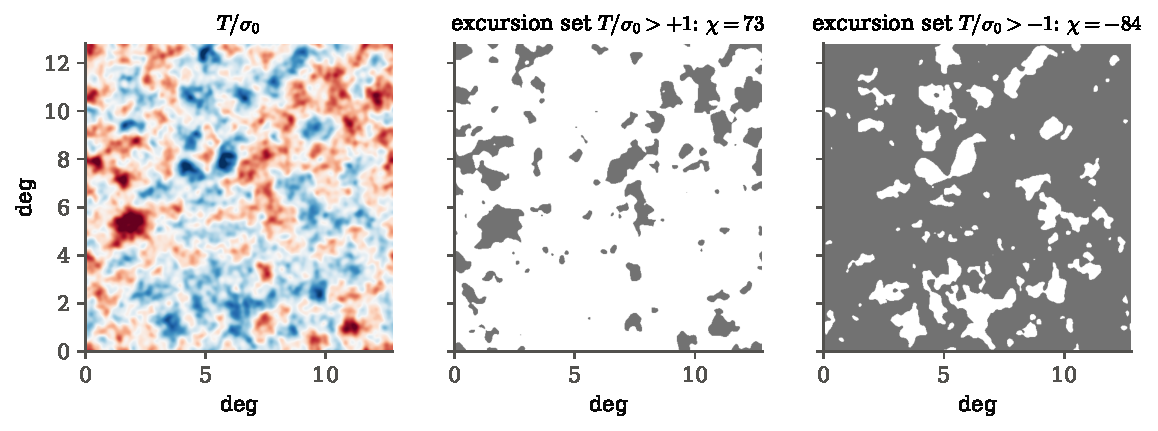
\includegraphics[width=\linewidth]{figures/chT3/patch_excursion.pdf}
\caption{Left: a simulated $\TaPatchDeg^\circ\times\TaPatchDeg^\circ$ patch of the CMB temperature, smoothed by a $10'$ beam, in units of its standard deviation $\sigma_0$. Middle: the pixels hotter than $+1\sigma_0$ form separate islands, with very few holes. Right: the pixels hotter than $-1\sigma_0$ form one connected region pierced by cold lakes, so holes outnumber pieces and the Euler characteristic is negative.}
\label{T3a:fig:patch}
\end{figure}

\paragraph{The question.} If we colour every point of the sky hotter than $\nu$ standard deviations, how much of the sky is coloured, how long is the coastline of the coloured region, and how many separate pieces does it have once its holes are subtracted? And for a Gaussian sky with a given $\Cell$, what should each of those three numbers be at each $\nu$?

\subsection{Excursion sets and their three numbers}
\label{T3a:sec:mf-def}

Write the temperature fluctuation in direction $\hat{\bm n}$ as $T(\hat{\bm n})$, measured from the mean, and its standard deviation over the sky as $\sigma_0$ (the subscript says it is the variance of the field itself, with no derivatives). The region of the sky where the field exceeds $\nu$ standard deviations is the \newterm{excursion set} at threshold $\nu$,
\begin{equation}
  Q_\nu=\{\hat{\bm n}\,:\,T(\hat{\bm n})>\nu\,\sigma_0\} .
  \label{T3a:eq:excursion}
\end{equation}
\Cref{T3a:fig:patch} shows two of them. In two dimensions a classical theorem of integral geometry (Hadwiger's) says that any summary of the shape of a region that adds up over disjoint pieces and does not care where the region sits or how it is turned is a combination of just three numbers \cite{SchmalzingGorski1998}: the area, the length of the boundary, and the Euler characteristic. These are the three \newterm{Minkowski functionals}.

\begin{workdef}[the Minkowski functionals of a map]
For a map $T$ on a patch of area $A$ and a threshold $\nu$, divide by the area to get densities:
\begin{itemize}[itemsep=1pt,leftmargin=1.2em]
  \item $v_0(\nu)$, the \emph{area fraction} \unpack{the fraction of pixels with $T>\nu\sigma_0$};
  \item $v_1(\nu)=\frac{1}{4A}\times$ the total length of the boundary of $Q_\nu$ \unpack{the factor $\frac14$ is a convention of integral geometry};
  \item $v_2(\nu)=\frac{1}{A}\times\chi(Q_\nu)$, where the \emph{Euler characteristic} $\chi$ is the number of separate pieces of $Q_\nu$ minus the number of holes in them \unpack{a hole is a cold region completely surrounded by hot sky}.
\end{itemize}
\emph{Operational:} $v_0$ is a pixel count. $v_1$ is the average of $|\nabla T|\,\delta(T-\nu\sigma_0)$ over the map, with the delta replaced by a narrow bin. $\chi$ is counted on the pixel grid as vertices minus edges plus faces of the union of the hot pixels (see the topology notes for why this alternating count gives pieces minus holes).
\end{workdef}

Why these three and not others? Each answers a physical question about the coloured region. The area fraction says how much of the sky is hotter than the threshold. The boundary length says how wiggly the coastline is, which is a statement about how fast the field changes in space. The Euler characteristic is the one number that does not change when the region is stretched or bent without tearing: it sees only connectivity. Its value is the same whether the island is round or elongated, so it is the most robust of the three to anything that distorts the map smoothly, a point that returns in \cref{T3a:sec:lensing}. On the full sky there is one more fact, from the Gauss--Bonnet theorem: a region that grows until it covers the whole sphere ends with $\chi=2$ (the Euler characteristic of a sphere), not $0$, so the full-sky count contains a small term proportional to the area, $\chi=V_2+V_0/(2\pi R^2)$ in the notation of \cite{SchmalzingGorski1998} (their eq.~7), where $V_0$ is the area, $V_2$ the integrated boundary curvature divided by $2\pi$ and $R$ the radius of the sphere.

\begin{figure}[htbp]
\centering
\begin{tikzpicture}[scale=0.9]
  \foreach \x/\lab/\cval in {0/{$\nu=-1$: one continent,\\ three lakes}/{$\chi=1-3=-2$},
                           5.2/{$\nu=0$: two pieces,\\ two holes}/{$\chi=2-2=0$},
                           10.4/{$\nu=+1$: three islands}/{$\chi=3-0=3$}} {
    \draw[faint] (\x,0) rectangle ++(4,4);
    \node[lbl,align=center,text width=4.4cm,anchor=north] at (\x+2,-0.2) {\lab};
    \node[lbl] at (\x+2,-1.5) {\cval};
  }
  \fill[bdryred!35,even odd rule] (0,0) rectangle (4,4) (1.0,2.9) circle (0.45) (2.8,1.1) circle (0.55) (3.1,3.1) circle (0.35);
  \draw[bdryred,thick] (1.0,2.9) circle (0.45) (2.8,1.1) circle (0.55) (3.1,3.1) circle (0.35);
  \fill[bdryred!35,even odd rule] (5.5,0.4) rectangle (7.6,3.6) (6.55,2.4) circle (0.45);
  \fill[bdryred!35,even odd rule] (8.0,0.4) rectangle (8.9,3.6) (8.45,1.2) circle (0.25);
  \draw[bdryred,thick] (5.5,0.4) rectangle (7.6,3.6) (6.55,2.4) circle (0.45) (8.0,0.4) rectangle (8.9,3.6) (8.45,1.2) circle (0.25);
  \fill[bdryred!35] (11.3,3.0) circle (0.45) (12.6,1.2) ellipse (0.7 and 0.4) (13.6,3.2) circle (0.3);
  \draw[bdryred,thick] (11.3,3.0) circle (0.45) (12.6,1.2) ellipse (0.7 and 0.4) (13.6,3.2) circle (0.3);
\end{tikzpicture}
\caption{Cartoon of excursion sets at three thresholds (shaded: hotter than the threshold). At a low threshold the hot region is one piece with cold lakes in it; at a high threshold it is a set of separate islands. The Euler characteristic, pieces minus holes, runs from negative to positive as the threshold rises.}
\label{T3a:fig:cartoon}
\end{figure}

\subsection{What a Gaussian sky predicts}
\label{T3a:sec:mf-gauss}

\emph{The area first.} The area fraction is the share of the sky where $T>\nu\sigma_0$. On a statistically homogeneous sky the average of a quantity over the sky equals its average over the ensemble of possible skies (ergodicity, \cref{7a:sec:ergodic}). So the expected area fraction is the probability that the field at one point exceeds the threshold. For a Gaussian field of mean zero and variance $\sigma_0^2$,
\begin{align}
  \E[v_0(\nu)]
  &\eqby{1}\Prob\big(T(\hat{\bm n})>\nu\sigma_0\big)
   \eqby{2}\int_{\nu\sigma_0}^{\infty}\frac{e^{-t^2/2\sigma_0^2}}{\sqrt{2\pi}\,\sigma_0}\,\dd t
   \eqby{3}\int_{\nu/\sqrt2}^{\infty}\frac{e^{-s^2}}{\sqrt\pi}\,\dd s
   \eqby{4}\tfrac12\operatorname{erfc}\!\big(\nu/\sqrt2\big) .
  \label{T3a:eq:v0}
\end{align}
\begin{explain}
  \item The sky average of the indicator of $Q_\nu$ equals its ensemble average at one point (ergodicity), and the average of an indicator is a probability.
  \item The one-point density of a Gaussian field.
  \item Substitute $s=t/(\sqrt2\sigma_0)$, so $\dd t=\sqrt2\sigma_0\,\dd s$.
  \item The definition $\operatorname{erfc}(x)=\frac{2}{\sqrt\pi}\int_x^\infty e^{-s^2}\dd s$.
\end{explain}

\paragraph{Example: the area above one standard deviation.} At $\nu=1$, \eqref{T3a:eq:v0} gives $\tfrac12\operatorname{erfc}(0.7071)=\TaVzeroOne$: about one sky pixel in six. The \TaNsimMF\ simulated patches of \cref{T3a:fig:mf} give \TaVzeroOneSim. Notice what $v_0$ does \emph{not} depend on: the spectrum. Only the one-point distribution enters, so $v_0$ is a test of the shape of the histogram of pixel values and nothing else.

\emph{Two numbers from the spectrum.} The boundary length and the Euler characteristic do depend on the spectrum, but only through two of its moments: the variance of the field, $\sigma_0^2=\langle T^2\rangle$, and the variance of its gradient, $\sigma_1^2=\langle|\nabla T|^2\rangle$ \cite{BBKS1986,SchmalzingGorski1998}. Both follow from $\Cell$. Write $T=\sum_{\ell m}\alm Y_{\ell m}$ with $\langle\alm a^*_{\ell'm'}\rangle=\Cell\,\delta_{\ell\ell'}\delta_{mm'}$ (\cref{7b:eq:alm-cov}). Then
\begin{align}
  \sigma_0^2=\langle T(\hat{\bm n})^2\rangle
  &\eqby{1}\sum_{\ell m}\Cell\,|Y_{\ell m}(\hat{\bm n})|^2
   \eqby{2}\sum_{\ell}\frac{2\ell+1}{4\pi}\,\Cell ,
  \label{T3a:eq:sigma0}\\
  \sigma_1^2=\langle|\nabla T|^2\rangle
  &\eqby{3}\Big\langle\frac{1}{4\pi}\int|\nabla T|^2\,\dd\Omega\Big\rangle
   \eqby{4}-\Big\langle\frac{1}{4\pi}\int T\,\nabla^2T\,\dd\Omega\Big\rangle\nonumber\\
  &\eqby{5}\frac{1}{4\pi}\sum_{\ell m}\ell(\ell+1)\langle|\alm|^2\rangle
   =\sum_{\ell}\frac{2\ell+1}{4\pi}\,\ell(\ell+1)\,\Cell .
  \label{T3a:eq:sigma1}
\end{align}
\begin{explain}
  \item Expand both factors of $T^2=T\,T^*$ (the field is real) and average; only $\ell=\ell'$, $m=m'$ survives.
  \item Addition theorem \eqref{7b:eq:addition} at coincident points, $\sum_m|Y_{\ell m}|^2=(2\ell+1)/4\pi$.
  \item On an isotropic sky the expectation at one point equals the expectation of the sky average.
  \item Integrate by parts on the sphere; there is no boundary term because the sphere has no edge.
  \item $\nabla^2Y_{\ell m}=-\ell(\ell+1)Y_{\ell m}$ and orthonormality of the $Y_{\ell m}$.
\end{explain}
A beam of window $b_\ell$ multiplies $\Cell$ by $b_\ell^2$ in both sums. The ratio has the dimension of an inverse angle squared, so it defines a correlation angle
\begin{equation}
  \theta_c\equiv\sigma_0/\sigma_1 ,
  \label{T3a:eq:thetac}
\end{equation}
the typical distance over which the field changes by one standard deviation. In flat-sky language, $\ell(\ell+1)\to|\bm\ell|^2$ and the sums become integrals over the plane of wave vectors.

\paragraph{Example: the correlation angle of a $10'$ map.} For the fiducial \textit{Planck} spectrum smoothed by a $10'$ beam, the full-sky sums give $\sigma_0=\TaSigZeroSky\,\mu$K and $\theta_c=\TaThetaCSky'$. On a $\TaPatchDeg^\circ$ patch the multipoles below $\ell\approx2\pi/\TaPatchDeg^\circ\approx28$ do not fit, so $\sigma_0$ drops to \TaSigZero\,$\mu$K and $\theta_c$ to $\TaThetaC'$. The lowest multipoles carry a large share of the variance but almost none of the gradient: they are the gentle, sky-wide tilts.

\emph{The boundary length: counting crossings.} The boundary of $Q_\nu$ is the set of points where $T=\nu\sigma_0$ exactly. Its length per unit area is the sky average of $|\nabla T|\,\delta(T-\nu\sigma_0)$: the delta function selects the points on the contour, and the factor $|\nabla T|$ converts ``a thin slab of threshold values of width $\dd T$'' into the length of contour it contains, since a steeper field crosses the slab in a narrower strip. By ergodicity the sky average is an ensemble average at one point, and at one point the value and the gradient of a homogeneous field are independent, because $\langle T\,\partial_iT\rangle=\tfrac12\partial_i\langle T^2\rangle=0$ and both are Gaussian. So the average factorises. On an isotropic sky the total gradient variance $\sigma_1^2$ splits equally between the two directions, so each component of $\nabla T$ has variance $s^2=\sigma_1^2/2$. The length $r=|\nabla T|$ of such a two-dimensional Gaussian vector has the Rayleigh density $(r/s^2)e^{-r^2/2s^2}$, with mean $\int_0^\infty (r^2/s^2)e^{-r^2/2s^2}\dd r=s\sqrt{\pi/2}$. Hence
\begin{align}
  \E[v_1(\nu)]
  &\eqby{1}\frac14\,\E\big[|\nabla T|\,\delta(T-\nu\sigma_0)\big]
   \eqby{2}\frac14\,\frac{e^{-\nu^2/2}}{\sqrt{2\pi}\,\sigma_0}\,\E|\nabla T|\nonumber\\
  &\eqby{3}\frac14\,\frac{e^{-\nu^2/2}}{\sqrt{2\pi}\,\sigma_0}\,\frac{\sigma_1}{\sqrt2}\sqrt{\frac\pi2}
   \eqby{4}\frac{1}{8\sqrt2\,\theta_c}\,e^{-\nu^2/2} .
  \label{T3a:eq:v1}
\end{align}
\begin{explain}
  \item The definition of $v_1$ (a quarter of the length per unit area) and the crossing-counting argument above.
  \item Independence of $T$ and $\nabla T$ at a point; the average of $\delta(T-\nu\sigma_0)$ is the one-point density of $T$ at $\nu\sigma_0$.
  \item The Rayleigh mean with $s=\sigma_1/\sqrt2$.
  \item $\frac{1}{\sqrt{2\pi}}\cdot\frac{1}{\sqrt2}\sqrt{\frac\pi2}=\frac{1}{2\sqrt2}$, and $\sigma_1/\sigma_0=1/\theta_c$.
\end{explain}
\emph{The Euler characteristic, stated.} The same reasoning applied to the number of hot regions minus holes needs the second derivatives of the field as well, and its derivation is in \cref{ch:12}. The result is
\begin{equation}
  \E[v_2(\nu)]=\frac{1}{(2\pi)^{3/2}}\,\frac{1}{2\theta_c^2}\;\nu\,e^{-\nu^2/2} ,
  \label{T3a:eq:v2}
\end{equation}
and \eqref{T3a:eq:v1} with \eqref{T3a:eq:v2} are the two curves referred to below as the Gaussian functionals. Here we read off what each factor means. The factor $e^{-\nu^2/2}$ is the reason a coastline exists at all: a boundary needs the field to be exactly at the threshold, and the probability density of that is proportional to $e^{-\nu^2/2}$. So boundaries and islands are rare at large $|\nu|$. The factor $1/\theta_c$ in $v_1$ turns ``crossings per unit of threshold'' into ``length per unit area'': a field that changes faster has more coastline. The factor $1/\theta_c^2$ in $v_2$ is one island per correlation area. Finally the factor $\nu$ makes $v_2$ odd. That follows from the symmetry of a Gaussian under $T\to-T$: the complement of the set $\{T>-\nu\sigma_0\}$ is the set $\{-T\ge\nu\sigma_0\}$, which has the same statistics as $Q_\nu$, and on a closed patch (a torus, or the plane far from edges) the Euler characteristic of a region and of its complement are opposite, because the pieces of one are the holes of the other. So $v_2(-\nu)=-v_2(\nu)$, and $v_2(0)=0$.

\paragraph{Example: how many hot spots above $2\sigma$?} At $\nu=2$ holes inside hot spots are rare, so $\chi$ counts the hot spots. On the full sky the Gaussian kinematic formula adds the sphere's own Euler characteristic times the area fraction to $4\pi$ times the density \eqref{T3a:eq:v2} \cite{SchmalzingGorski1998}:
\begin{align*}
  \E[\chi_{\rm sky}(2)]
  &\eqby{1}4\pi\,\frac{1}{(2\pi)^{3/2}}\,\frac{1}{2\theta_c^2}\,2e^{-2}
   +2\cdot\tfrac12\operatorname{erfc}(\sqrt2)\\
  &\eqby{2}4\pi\times0.0635\times\frac{1}{2\,(3.90\times10^{-3})^2}\times0.271+2\times0.0228
   \;\approx\;7.1\times10^{3} .
\end{align*}
\begin{explain}
  \item The density \eqref{T3a:eq:v2} at $\nu=2$ times the area $4\pi$ of the sphere, plus $\chi(S^2)=2$ times $\E[v_0(2)]$ from \eqref{T3a:eq:v0}.
  \item $(2\pi)^{-3/2}=0.0635$, $\theta_c=\TaThetaCSky'=3.90\times10^{-3}$\,rad, $2e^{-2}=0.271$. The second term is negligible.
\end{explain}
The unrounded evaluation in \pyname{01_excursion_mfs.py} gives \TaHotSpotsSky. A $10'$ map of the whole sky has several thousand hot spots above two standard deviations; a sky with a hundred more or a hundred fewer would be a statement about physics.

\subsection{Checking the formulas on simulated skies}
\label{T3a:sec:mf-code}

To see the formulas at work we simulate \TaNsimMF\ flat patches of $\TaPatchDeg^\circ\times\TaPatchDeg^\circ$, with $\TaPixArcmin'$ pixels and the fiducial lensed spectrum smoothed by a $10'$ beam, and measure all three functionals at 41 thresholds. The area fraction is a pixel count, the boundary length uses the binned-delta average of $|\nabla T|$, and the Euler characteristic is counted on the pixel grid:
\pyfile[firstline=106,lastline=119]{code/chT3/lib_t3.py}{Counting pieces minus holes on the pixel grid}
Each pixel above the threshold is a closed square. The function counts the squares ($F$), the pixel edges that belong to at least one of them ($E$), and the pixel corners that belong to at least one of them ($V$); the alternating sum $V-E+F$ is the Euler characteristic of their union. The rolls make the patch periodic, so the patch is a torus and has no edge to correct for. On one map the count agrees exactly with \pyname{skimage.measure.euler_number} (\TaEulerOurs\ and \TaEulerSkimage), the library routine the research literature uses.

\begin{figure}[htbp]
\centering
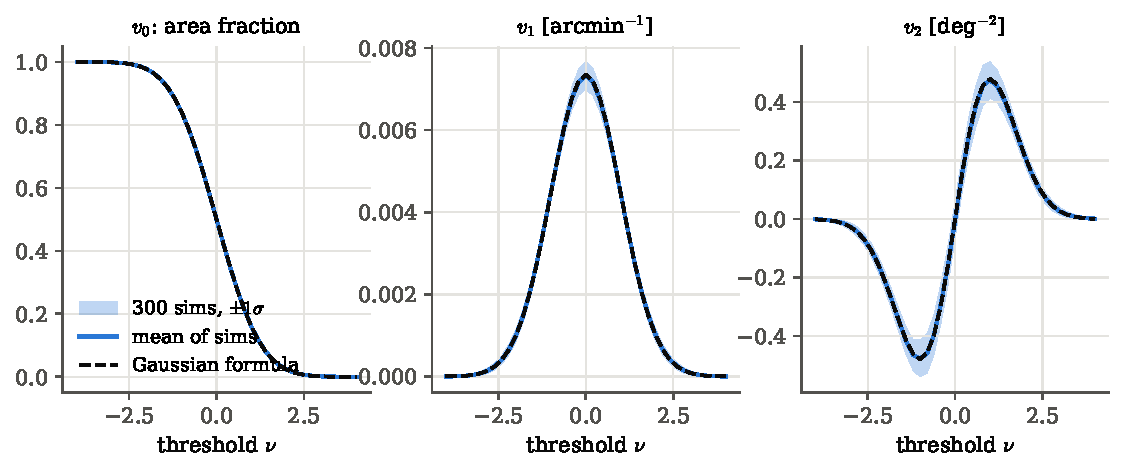
\includegraphics[width=\linewidth]{figures/chT3/mf_gaussian.pdf}
\caption{The three Minkowski functionals of simulated Gaussian CMB patches ($10'$ beam) against the threshold. The band is the spread of single patches, the solid line their mean, and the dashed line the Gaussian formulas \eqref{T3a:eq:v0} and \eqref{T3a:eq:v1},~\eqref{T3a:eq:v2} with $\sigma_0$ and $\sigma_1$ computed from the spectrum. The Euler characteristic changes sign at $\nu=0$: islands above, lakes below.}
\label{T3a:fig:mf}
\end{figure}

\Cref{T3a:fig:mf} shows the result. The mean of the simulations lies on the Gaussian curves; the largest departure of the mean Euler characteristic from the formula is \TaChiDevPct\% of its peak, against a Monte Carlo error of \TaChiErrPct\% on the mean. The bands are wide: a single $\TaPatchArea$-square-degree patch has a peak Euler characteristic near \TaChiPeakPatch, and the patch-to-patch scatter is many times larger than the error on the mean. That scatter is the sampling distribution of the statistic, and it is what \cref{ch:12} estimates by Monte Carlo to turn a measured curve into a test.

\begin{pitfall}[Thresholds in units of which $\sigma_0$?]
The formulas use the true $\sigma_0$ of the ensemble. A map only gives its own sample standard deviation, which differs from patch to patch (a $\TaPatchArea\,{\rm deg}^2$ patch misses all the variance at $\ell\lesssim28$). Normalising each map by its own standard deviation removes most of the scatter in the \emph{amplitude} of the curves and leaves their shape, which is why \textit{Planck} does it (\cref{T3a:sec:planck}). Whichever choice is made, the simulations must make the same one.
\end{pitfall}

Real maps are not Gaussian random fields drawn on a computer, and the functionals are just as easy to compute on any surface. \cite{SchmalzingGorski1998} show them for the Earth's topography binned onto a sky map: the curves change sharply at the depth of the ocean floor and at sea level, the Euler characteristic dips where the mid-ocean ridges emerge as long connected ranges, and nothing about them looks like \eqref{T3a:eq:v1},~\eqref{T3a:eq:v2}. A strongly non-Gaussian surface announces itself immediately. The cosmological question is the opposite one: how small a departure from the Gaussian curves can be detected, and what would cause it.
\section{What a skewed sky and a lensed sky change}
\label{T3a:sec:nongauss}

The simplest inflationary models make the primordial fluctuations almost exactly Gaussian. Models with more than one field can leave a small quadratic piece. The standard way of writing it, used by \textit{Planck}, is the \newterm{local model} \cite{Planck2018IX}
\begin{equation}
  \Phi(\bm x)=\phi(\bm x)+f_{\rm NL}\big[\phi^2(\bm x)-\langle\phi^2\rangle\big],
  \label{T3a:eq:local}
\end{equation}
where $\phi$ is a Gaussian field, $\Phi$ is the primordial potential (Bardeen's potential, $\Phi=\tfrac35\zeta$ on super-horizon scales, with $\zeta$ the comoving curvature perturbation; see the cosmology notes), and $f_{\rm NL}$ is a number that measures how much of the square is mixed in. Subtracting $\langle\phi^2\rangle$ keeps the mean of $\Phi$ zero. Because $\phi\sim10^{-5}$, even $f_{\rm NL}\sim10$ makes the quadratic term a part in $10^{4}$ of the linear one. The question is what such a term does to the three curves of \cref{T3a:fig:mf}. A second question runs alongside it. Every CMB photon has been deflected by a couple of arcminutes on its way to us; does that change the curves?

\paragraph{The question.} If the sky is slightly skewed, which of the three Minkowski functionals move, by how much, and how much of the move tells us about the physics that produced the skewness rather than about the histogram of pixel values? And what does lensing do to the same three numbers?

\subsection{The first correction to the Gaussian curves}
\label{T3a:sec:matsubara}

A mildly non-Gaussian field is described, to first order, by its three-point averages. For the Minkowski functionals in two dimensions only three such averages matter \cite{Matsubara2003} (his eqs.~2.61--2.63 with $d=2$). Measured in units of $\sigma_0$, and with $\theta_c=\sigma_0/\sigma_1$ the correlation angle of \eqref{T3a:eq:thetac}, they are
\begin{equation}
  S^{(0)}\sigma_0=\frac{\langle T^3\rangle}{\sigma_0^3},\qquad
  S^{(1)}\sigma_0=-\frac34\,\frac{\langle T^2\,\nabla^2T\rangle}{\sigma_0\,\sigma_1^2},\qquad
  S^{(2)}\sigma_0=-3\,\frac{\langle|\nabla T|^2\,\nabla^2T\rangle\,\sigma_0}{\sigma_1^4} .
  \label{T3a:eq:skewpar}
\end{equation}
The first is the ordinary skewness of the histogram of pixel values: positive when the hot tail is longer than the cold one. The other two, the \newterm{skewness parameters} of the derivatives, say whether hot regions differ from cold ones in how steep and how curved they are. All three vanish for a Gaussian field. To first order in them, Matsubara's result (his eq.~3.48, $d=2$) reads
\begin{align}
  \E[v_0(\nu)]&=\tfrac12\operatorname{erfc}\!\big(\nu/\sqrt2\big)
     +\frac{e^{-\nu^2/2}}{\sqrt{2\pi}}\,\frac{S^{(0)}\sigma_0}{6}\,H_2(\nu),\nonumber\\
  \E[v_1(\nu)]&=\frac{1}{8\sqrt2\,\theta_c}\,e^{-\nu^2/2}\Big\{1+\Big[\frac{S^{(0)}}{6}H_3(\nu)+\frac{S^{(1)}}{3}H_1(\nu)\Big]\sigma_0\Big\},
  \label{T3a:eq:matsubara}\\
  \E[v_2(\nu)]&=\frac{1}{(2\pi)^{3/2}}\,\frac{1}{2\theta_c^2}\,e^{-\nu^2/2}\Big\{H_1(\nu)+\Big[\frac{S^{(0)}}{6}H_4(\nu)+\frac{2S^{(1)}}{3}H_2(\nu)+\frac{S^{(2)}}{3}\Big]\sigma_0\Big\},\nonumber
\end{align}
with the Hermite polynomials $H_n(\nu)=e^{\nu^2/2}(-\dd/\dd\nu)^ne^{-\nu^2/2}$, that is $H_1=\nu$, $H_2=\nu^2-1$, $H_3=\nu^3-3\nu$, $H_4=\nu^4-6\nu^2+3$. Setting the $S^{(a)}$ to zero gives back \eqref{T3a:eq:v0} and \eqref{T3a:eq:v1},~\eqref{T3a:eq:v2}. The derivation is the Gaussian one of \cref{ch:12} with the joint density of the field and its derivatives expanded one order beyond the Gaussian (an Edgeworth expansion).

\subsection{A pointwise distortion only relabels the threshold}
\label{T3a:sec:relabel}

\emph{The claim in words.} Suppose the observed map is a fixed increasing function of a Gaussian map, $T=g(u)$, applied pixel by pixel. Then the region where $T$ exceeds $t$ is exactly the region where $u$ exceeds $g^{-1}(t)$. The two maps have the same excursion sets; only the labels on the thresholds differ. So every functional of $T$ at threshold $t$ is the Gaussian functional of $u$ at threshold $g^{-1}(t)$, and the whole non-Gaussian correction is a sideways shift of the curves.

\begin{figure}[htbp]
\centering
\begin{tikzpicture}
\begin{axis}[width=7.2cm,height=5.4cm,xmin=-2.5,xmax=2.5,ymin=-2.6,ymax=4.4,
  xlabel={Gaussian value $u$},ylabel={observed value $T=g(u)$},
  axis lines=left,tick label style={font=\scriptsize},label style={font=\small},
  legend style={font=\scriptsize,draw=none,at={(0.02,0.98)},anchor=north west}]
  \addplot[formblue,thick,domain=-2.5:2.5,samples=100] {x+0.15*(x^2-1)};
  \addlegendentry{$g(u)=u+a(u^2-1)$, $a=0.15$}
  \addplot[softgray,dashed,domain=-2.5:2.5] {x};
  \addlegendentry{$T=u$ (Gaussian)}
  \pgfmathsetmacro{\ustar}{(-1+sqrt(1+4*0.15*(2+0.15)))/(2*0.15)}
  \draw[bdryred,thick] (axis cs:-2.5,2) -- (axis cs:\ustar,2) -- (axis cs:\ustar,-2.6);
  \addplot[only marks,mark=*,mark size=1.6pt,bdryred] coordinates {(\ustar,2)};
\end{axis}
\end{tikzpicture}
\caption{A pointwise, increasing distortion of the values. The threshold $T=2$ on the observed map (horizontal red line) picks out exactly the pixels with $u>g^{-1}(2)\approx1.71$ on the Gaussian map (vertical red line). The excursion set is the same set of pixels; only the number attached to the threshold has changed.}
\label{T3a:fig:relabel}
\end{figure}

\paragraph{Example: the relabelling reproduces Matsubara's correction.} Take $T=u+a(u^2-1)$ with $u$ Gaussian of unit variance and $a$ small (\cref{T3a:fig:relabel}). Its skewness is
\begin{align*}
  \langle T^3\rangle
  \eqby{1}\langle u^3\rangle+3a\,\langle u^2(u^2-1)\rangle+O(a^2)
  \eqby{2}0+3a\,(3-1)=6a ,
\end{align*}
\begin{explain}
  \item Expand the cube and keep terms of first order in $a$.
  \item Odd Gaussian moments vanish, $\langle u^4\rangle=3$ and $\langle u^2\rangle=1$.
\end{explain}
so $S^{(0)}\sigma_0=6a$, and a calculation of the same kind (or the simulation below) gives $S^{(1)}\sigma_0=S^{(2)}\sigma_0=6a$ as well. Now do it the other way. The threshold $\nu$ on $T$ corresponds to $u_\nu=g^{-1}(\nu)=\nu-a(\nu^2-1)+O(a^2)$, so
\begin{align*}
  v_2^T(\nu)=v_2^G(u_\nu)
  &\eqby{1}v_2^G(\nu)-a(\nu^2-1)\,\frac{\dd v_2^G}{\dd\nu}
   \eqby{2}v_2^G(\nu)+\frac{1}{(2\pi)^{3/2}}\frac{1}{2\theta_c^2}\,e^{-\nu^2/2}\,a\,(\nu^2-1)^2\\
  &\eqby{3}v_2^G(\nu)+\frac{1}{(2\pi)^{3/2}}\frac{1}{2\theta_c^2}\,e^{-\nu^2/2}\,
   \Big[\frac{6a}{6}H_4+\frac{2\cdot6a}{3}H_2+\frac{6a}{3}\Big] .
\end{align*}
\begin{explain}
  \item Taylor expansion to first order in the shift $-a(\nu^2-1)$.
  \item $\frac{\dd}{\dd\nu}(\nu e^{-\nu^2/2})=(1-\nu^2)e^{-\nu^2/2}$, so the product of the two minus signs is $+a(\nu^2-1)^2$.
  \item $H_4+4H_2+2=\nu^4-6\nu^2+3+4\nu^2-4+2=(\nu^2-1)^2$.
\end{explain}
The last line is \eqref{T3a:eq:matsubara} with all three skewness parameters equal to $6a$. For a pointwise distortion the perturbative formula is nothing but the relabelling.

\emph{Removing the relabelling.} The relabelling can be undone without knowing $g$. Instead of the threshold $\nu$, label each excursion set by the area it covers: define the \newterm{area threshold} $\nu_A$ by $\tfrac12\operatorname{erfc}(\nu_A/\sqrt2)=$ the measured area fraction. A pointwise increasing distortion keeps the order of the pixel values, so the set covering a given fraction of the sky is the same set before and after it. At fixed $\nu_A$ the three functionals of $T=g(u)$ are therefore exactly those of $u$. In Matsubara's expansion this shows up as follows: rewritten in terms of $\nu_A$, the corrections contain only the differences $S^{(1)}-S^{(0)}$ and $S^{(2)}-S^{(0)}$ \cite{Matsubara2003} (his eq.~3.54), which vanish when the three are equal. What is left at fixed area fraction is information about how the skewness is shared between the field and its slopes and curvatures, and that information can only come from physics that couples neighbouring points.

\subsection{Testing it on two skewed skies}
\label{T3a:sec:ng-code}

\pyname{02_nongaussian_mfs.py} builds two kinds of skewed patch, both with the smoothed CMB spectrum shape of \cref{T3a:sec:mf-code}, and with amplitudes exaggerated so that the effect stands out in \TbNsim\ patches. The \emph{local} sky is $T=u+a(u^2-1)$ with $a=\TbA$; the code measures $S^{(0)}\sigma_0,S^{(1)}\sigma_0,S^{(2)}\sigma_0=\TbLocSzero,\TbLocSone,\TbLocStwo$, against $6a=\TbSixA$. The \emph{non-local} sky applies the same quadratic term, with coefficient $\TbB$, to a scale-invariant field $\phi$ (equal power per logarithmic interval of $\ell$, like the primordial potential) and then filters the result with the transfer function that turns $\phi$'s spectrum into the CMB one. The filter mixes neighbouring points, as the physics between the end of inflation and last scattering does, and the measured parameters are no longer equal: $\TbNlSzero,\TbNlSone,\TbNlStwo$.

\begin{figure}[htbp]
\centering
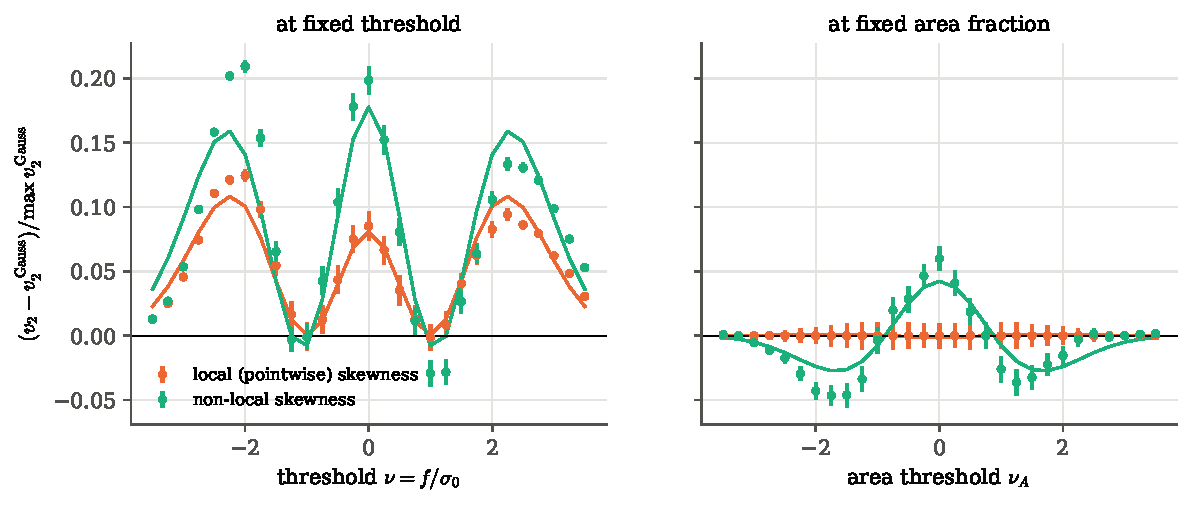
\includegraphics[width=\linewidth]{figures/chT3/ng_mfs.pdf}
\caption{Change of the Euler characteristic density of two skewed skies from the Gaussian one, in units of the peak of the Gaussian curve. Points: \TbNsim\ simulated patches; lines: Matsubara's first-order formula with the measured skewness parameters. Left, at fixed threshold $\nu$: the local sky moves by up to about a tenth of the peak, the non-local one by up to about a fifth. Right, at fixed area fraction: the pointwise (local) distortion disappears exactly, the non-local one does not.}
\label{T3a:fig:ng}
\end{figure}

\Cref{T3a:fig:ng} shows the result. At fixed threshold the local sky shifts by up to \TbLocMaxShiftPct\% of the peak, with the shape $(\nu^2-1)^2$ predicted above. At fixed area fraction the shift is \TbLocAreaMaxPct\%: the same pixels, the same sets, the same counts, realisation by realisation. The non-local sky keeps a shift of up to \TbNlAreaMaxPct\% of the peak at fixed area fraction, against a Monte Carlo error of \TbErrPct\% (the non-local and Gaussian patches are independent draws, so both errors enter), and the first-order formula follows it roughly. Near $\nu_A=-2$ the points and the formula differ by \TbNlResPct\% of the peak, \TbNlResSig\ times that error, too few for \TbNsim\ patches to pin down. A difference there would be no surprise: $S^{(0)}\sigma_0\approx0.5$ is not small, and the formula keeps only the first order.

\paragraph{Example: what the real $f_{\rm NL}$ does on large scales.} On the largest angular scales the temperature is set by the potential at last scattering alone, $\Delta T/T=-\Phi/3$ (the Sachs--Wolfe limit; see the cosmology notes). Insert the local model \eqref{T3a:eq:local} and write the Gaussian part of the temperature as $t=-\phi/3$, so that $\phi=-3t$:
\begin{align*}
  \frac{\Delta T}{T}=-\frac{\Phi}{3}
  &\eqby{1}-\frac{\phi}{3}-\frac{f_{\rm NL}}{3}\big(\phi^2-\langle\phi^2\rangle\big)
   \eqby{2}t-3f_{\rm NL}\big(t^2-\langle t^2\rangle\big)
   \eqby{3}\sigma_t\Big[u-3f_{\rm NL}\sigma_t\,(u^2-1)\Big] .
\end{align*}
\begin{explain}
  \item Substitute \eqref{T3a:eq:local}.
  \item $\phi=-3t$, so $\phi^2=9t^2$ and $-\tfrac{f_{\rm NL}}{3}\cdot9=-3f_{\rm NL}$.
  \item Write $t=\sigma_t u$ with $u$ of unit variance.
\end{explain}
This is the local toy with $a=-3f_{\rm NL}\sigma_t$. Two conclusions follow. First, the sign: a positive $f_{\rm NL}$ gives a negative skewness $6a$, so the cold spots of the Sachs--Wolfe sky are the more extreme ones. Second, the size: the large-angle temperature has $\sigma_t\approx2\times10^{-5}$, so $f_{\rm NL}=5$ gives $|6a|\approx18\times5\times2\times10^{-5}\approx2\times10^{-3}$, a shift of the Euler characteristic of order $0.1$--$0.2\%$ of its peak, and at fixed area fraction none at all. On scales where the temperature is a pointwise function of the potential, the Minkowski functionals at fixed area fraction are blind to local $f_{\rm NL}$; the signal that survives comes from the acoustic scales, where the transfer is non-local, and it is small there too. This is why \textit{Planck} measures $f_{\rm NL}$ with the bispectrum, the optimal statistic for a known three-point shape, and uses the Minkowski functionals as a model-independent check (\cref{T3a:sec:planck}).

\subsection{Lensing leaves the one-point distribution alone}
\label{T3a:sec:lens-mf}

Lensing moves the photons arriving in direction $\hat{\bm n}$ so that we see the last-scattering surface at a neighbouring point, $\tilde T(\hat{\bm n})=T(\hat{\bm n}+\bm\alpha)$, with a deflection $\bm\alpha$ of a couple of arcminutes that is coherent over a couple of degrees \cite{LewisChallinor2006} (their \S1.2). It does not change the photons' energies, so it conserves surface brightness: every temperature we see in the lensed sky is a temperature that existed on the unlensed one, seen in a slightly different direction. For a statistically homogeneous sky the lensed one-point distribution is therefore the unlensed one, and in particular the variance is unchanged, $\tilde\sigma_0=\sigma_0$ (their eq.~4.30). By \eqref{T3a:eq:v0} the area functional $v_0(\nu)$ is untouched. The gradient variance is not: lensing shears and magnifies the image, moving power to smaller scales, so $\tilde\sigma_1>\sigma_1$. Plugged into \eqref{T3a:eq:v1},~\eqref{T3a:eq:v2}, that would predict more coastline and more islands. Whether there really are more islands is a question about topology, and \cref{T3a:sec:lensing} answers it: a smooth remapping cannot change how many islands there are.

\paragraph{Example: lensing that looks like $f_{\rm NL}$.} The deflection is produced by the same large-scale structure that, through the integrated Sachs--Wolfe effect, adds a little to the large-angle temperature. The two are correlated, and the correlation produces a three-point signal in the observed temperature whose shape resembles the local one. \textit{Planck}'s temperature-only estimate of local $f_{\rm NL}$ is $6.7\pm5.6$ before subtracting the expected lensing contribution and $-0.5\pm5.6$ after it \cite{Planck2018IX} (their Table~5, KSW estimator, \texttt{SMICA}). A lensed sky is, for three-point statistics, a slightly non-Gaussian sky with a known shape, and an analysis that forgets it reports a spurious $f_{\rm NL}$ of about one standard deviation.
\section{Polarization patterns and their singularities}
\label{T3a:sec:polarization}

The CMB is linearly polarized at the level of a few per cent of its anisotropy. At each point of the sky the polarization is described by two Stokes parameters, $Q$ and $U$, measured with respect to a pair of axes drawn on the sky at that point. Draw a short stick at each point, along the direction of the polarization. The stick has a direction but no arrowhead: turning it by $180^\circ$ gives the same stick, because a polarization direction is the orientation of an oscillating electric field, not the direction of a vector. In the language of \cite{VachaspatiLue2003}, the sky is covered with headless rods, like the molecules of a thin film of nematic liquid crystal, and such patterns have point defects. Wherever $Q$ and $U$ both vanish, the stick has no direction at all. Walk around such a point and the sticks turn steadily, by half a turn in one sense or the other. These points are the \newterm{polarization singularities}.

\paragraph{The question.} Where does the polarization vanish? What does the pattern of sticks look like around such a point, and why only half a turn? How many such points does a Gaussian polarization map with given $C_\ell^{EE}$ and $C_\ell^{BB}$ have per square degree, and does their arrangement carry information that the spectra do not?

\subsection{Headless sticks and a half-integer index}
\label{T3a:sec:index}

\emph{From $Q$ and $U$ to a stick.} The polarization at a point is a symmetric, trace-free $2\times2$ matrix \cite{VachaspatiLue2003} (their eq.~1),
\begin{equation}
  \mathsf P=\begin{pmatrix}Q&U\\U&-Q\end{pmatrix},
  \qquad
  \frac{\mathsf P}{2P}=\hat{\bm m}\hat{\bm m}^{\mathsf T}-\tfrac12\Id,\qquad P=\sqrt{Q^2+U^2},
  \label{T3a:eq:Pmatrix}
\end{equation}
with $\hat{\bm m}=(\cos\alpha,\sin\alpha)$ the unit vector along the stick. Multiplying out $\hat{\bm m}\hat{\bm m}^{\mathsf T}-\frac12\Id$ gives the matrix with entries $\frac12\cos2\alpha$ and $\frac12\sin2\alpha$, so $Q=P\cos2\alpha$ and $U=P\sin2\alpha$ \cite{HutererVachaspati2005} (their eq.~2). The vector $\hat{\bm m}$ enters twice, so $\hat{\bm m}$ and $-\hat{\bm m}$ give the same matrix: that is the missing arrowhead. In complex notation,
\begin{equation}
  Q+iU=P\,e^{2i\alpha},\qquad \alpha=\tfrac12\arg(Q+iU),
  \label{T3a:eq:alpha}
\end{equation}
and rotating the reference axes by an angle $\psi$ changes $\alpha$ by $-\psi$ and the pair $(Q,U)$ by $-2\psi$. That factor two is what is meant by calling the polarization a spin-2 quantity.

\begin{workdef}[polarization singularity and its index]
A \emph{polarization singularity} is a point where $Q=U=0$ \unpack{the polarized intensity $P$ vanishes, so the stick direction $\alpha$ is undefined}. Its \emph{index} is the number of turns the stick makes along a small loop $\Gamma$ around it,
\begin{equation*}
  W_\Gamma=\frac{1}{2\pi}\oint_\Gamma \dd\alpha ,
\end{equation*}
with $\dd\alpha$ the change of the stick angle along the loop \cite{VachaspatiLue2003} (their eq.~5). \emph{Operational:} on a pixel grid, add the changes of $\arg(Q+iU)$ around each $2\times2$ block of pixels, each change taken the short way round the circle; the total is $2\pi n$, and the index is $n/2$.
\end{workdef}

\emph{Why the index is a half-integer.} Go once around the loop. The complex number $Q+iU$ comes back to its starting value, so its phase $2\alpha$ has changed by a whole number of turns, $2\pi n$. The stick angle $\alpha$ has therefore changed by $\pi n$, and $W_\Gamma=n/2$. A stick that has turned by $\pi$ looks exactly as it did at the start, so half-integers are allowed, which they would not be for arrows. \emph{Why $\pm\frac12$ is the usual value.} Near a generic zero both $Q$ and $U$ vanish linearly. The simplest such patterns are $Q+iU=x+iy$ and $Q+iU=x-iy$, with $(x,y)$ measured from the zero. In polar coordinates $x+iy=re^{i\theta}$, the first gives $\alpha=\theta/2$: the stick turns half a turn in the same sense as the loop, index $+\frac12$. The second gives $\alpha=-\theta/2$: half a turn against it, index $-\frac12$. These two patterns, drawn in \cref{T3a:fig:defects}, are the fundamental singularities; a general linear zero, $Q+iU=c_1(x+iy)+c_2(x-iy)$, has the index of whichever coefficient is larger in modulus. The index $\pm1$ patterns often drawn in the CMB literature (radial and circular patterns, and saddles) are pairs of fundamental singularities sitting on top of each other \cite{VachaspatiLue2003,HutererVachaspati2005}, which a random field produces only by accident.

\begin{figure}[htbp]
\centering
\begin{tikzpicture}[scale=1.0]
  \foreach \cx/\sg/\lab in {0/1/{index $+\tfrac12$: $Q+iU=x+iy$}, 6/-1/{index $-\tfrac12$: $Q+iU=x-iy$}} {
    \begin{scope}[xshift=\cx cm]
      \foreach \x in {-2,-1.5,...,2} {
        \foreach \y in {-2,-1.5,...,2} {
          \pgfmathsetmacro{\rr}{sqrt(\x*\x+\y*\y)}
          \ifdim \rr pt>0.3pt
            \pgfmathsetmacro{\ang}{0.5*\sg*atan2(\y,\x)}
            \draw[formblue,thick] ({\x-0.2*cos(\ang)},{\y-0.2*sin(\ang)}) -- ({\x+0.2*cos(\ang)},{\y+0.2*sin(\ang)});
          \fi
        }
      }
      \draw[bdryred,thick] (0,0) circle (0.9);
      \node[bdryred] at (0,0) {$\times$};
      \node[lbl] at (0,-2.6) {\lab};
    \end{scope}
  }
\end{tikzpicture}
\caption{The two fundamental polarization singularities. Each stick is drawn along $\alpha=\pm\frac12\arg(x+iy)$ at its grid point, and the cross marks the zero. Following the sticks once around the red loop, they turn half a turn with the loop (left) or half a turn against it (right).}
\label{T3a:fig:defects}
\end{figure}

\emph{The total index.} On a closed surface the indices of all singularities of a line field add up to the Euler characteristic of the surface (the Poincar\'e--Hopf theorem; see the topology notes). The sky is a sphere, so the indices of all the singularities on the full sky add up to $+2$ \cite{VachaspatiLue2003}: it is impossible to comb the polarization smoothly over the whole sky. With thousands of singularities of each sign this excess of four half-charges is negligible \cite{HutererVachaspati2005}. On a periodic flat patch, a torus, the total is exactly $0$.

\subsection{How many singularities a Gaussian sky has}
\label{T3a:sec:density}

\emph{The counting idea.} Look at a tiny square of sky of area $\dd A$. The map $(x,y)\mapsto(Q,U)$ sends it to a tiny parallelogram in the $(Q,U)$ plane of area $|\det J|\,\dd A$, where $J$ is the Jacobian matrix with rows $\nabla Q$ and $\nabla U$. The square contains a zero exactly when that parallelogram contains the origin of the $(Q,U)$ plane. So the expected number of zeros per unit area is the probability density of $(Q,U)$ at the origin, times the average area factor:
\begin{align}
  n
  &\eqby{1}p_{Q,U}(0,0)\;\E\,|\det J|
   \eqby{2}\frac{1}{2\pi\sigma_0^2}\;\E\,|\det J|
   \eqby{3}\frac{1}{2\pi\sigma_0^2}\cdot\frac{\sigma_1^2}{2}
   =\frac{\sigma_1^2}{4\pi\sigma_0^2} ,
  \label{T3a:eq:density}
\end{align}
\begin{explain}
  \item For a statistically homogeneous Gaussian field the value and the gradient at the same point are uncorrelated, hence independent: $\langle Q\,\partial_xQ\rangle=\frac12\partial_x\langle Q^2\rangle=0$, and similarly for the other pairs.
  \item For isotropic polarization $Q$ and $U$ are uncorrelated at a point with equal variances $\sigma_0^2$, so their joint density at the origin is $1/(2\pi\sigma_0^2)$.
  \item Shown just below, with $\sigma_1^2=\langle|\nabla Q|^2\rangle=\langle|\nabla U|^2\rangle$.
\end{explain}
\emph{The average area factor.} Write $\det J=|\nabla Q|\,|\nabla U|\,\sin\theta$, with $\theta$ the angle between the two gradients. For isotropic polarization the four derivatives are independent Gaussians of equal variance $s^2=\sigma_1^2/2$ (a direction-averaged statement checked by \pyname{03_polarization.py}). Each gradient is then a two-dimensional Gaussian vector, whose length has the Rayleigh mean $s\sqrt{\pi/2}$ (the integral done for \eqref{T3a:eq:v1}), and whose direction is uniform and independent of the other. So $\E|\det J|=(s\sqrt{\pi/2})^2\cdot\E|\sin\theta|=s^2\frac{\pi}{2}\cdot\frac{2}{\pi}=s^2=\sigma_1^2/2$.

Both variances come from the spectra exactly as in \eqref{T3a:eq:sigma0} and \eqref{T3a:eq:sigma1}, now with $C_\ell^P=C_\ell^{EE}+C_\ell^{BB}$ in place of $\Cell$ ($Q$ and $U$ each carry half of the total $E$ plus $B$ power, and the half cancels in the ratio). The ratio is an average of $\ell(\ell+1)$ weighted by the polarization power, so the expected number of singularities on the full sky is
\begin{equation}
  N_{\rm sky}=4\pi n=\frac{\sum_\ell(2\ell+1)\,\ell(\ell+1)\,C_\ell^P}{\sum_\ell(2\ell+1)\,C_\ell^P}\equiv\big\langle\ell(\ell+1)\big\rangle_P .
  \label{T3a:eq:Nsky}
\end{equation}
In words: one singularity per patch of area $4\pi\theta_P^2$, where $\theta_P=\sigma_0/\sigma_1$ is the correlation angle of the polarization. (On the sphere the spin-2 nature of $Q+iU$ changes $\ell(\ell+1)$ to $\ell(\ell+1)-4$ at the lowest multipoles, which does not matter for the counts below.)

\paragraph{Example: a $10'$ polarization map.} For the fiducial $C_\ell^{EE}+C_\ell^{BB}$ smoothed by a $10'$ beam, \eqref{T3a:eq:density} predicts \TcPred\ singularities in a $\TaPatchDeg^\circ\times\TaPatchDeg^\circ$ patch, about \TcPerDeg\ per square degree. The \TcNsim\ simulated patches of \cref{T3a:fig:polstats} have \TcMean\ on average, off the prediction by $\TcMeanDevPct\%$, which is \TcMeanDevSig\ standard errors of the mean but tiny next to the spread from patch to patch. That spread is $\TcSd\pm\TcSdErr$, close to the Poisson value $\sqrt{N}=\TcSdPoisson$. The net index of every patch is exactly zero, as Poincar\'e--Hopf requires on a torus.

\begin{figure}[htbp]
\centering
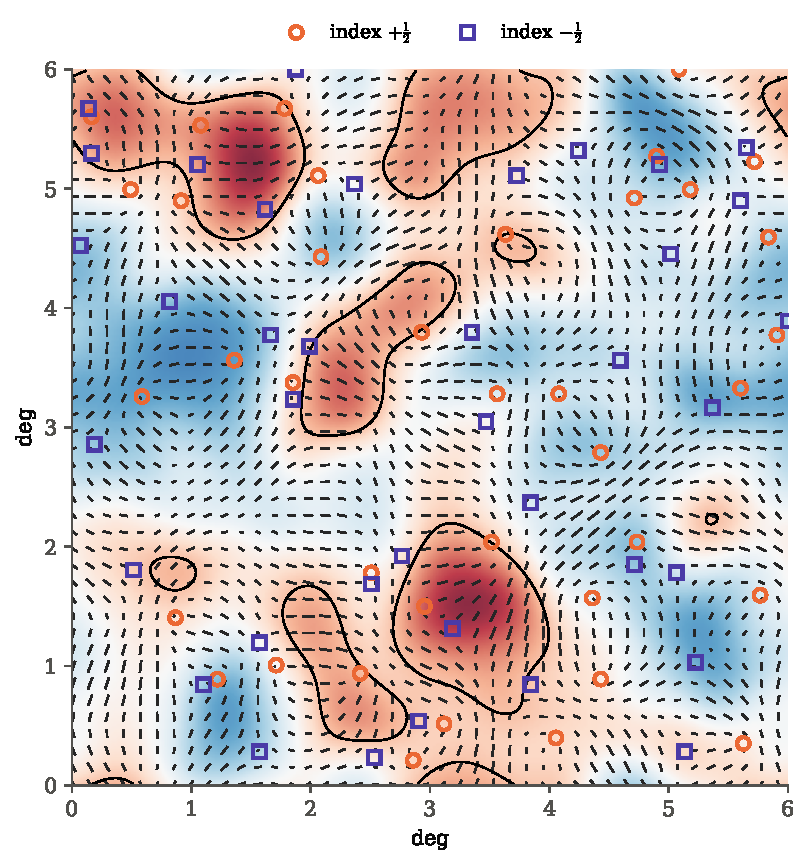
\includegraphics[width=0.78\linewidth]{figures/chT3/pol_patch.pdf}
\caption{A simulated $6^\circ\times6^\circ$ patch of the CMB with a $30'$ beam: temperature in colour (units of its standard deviation), the boundary of the excursion set $T>+1\sigma_0$ as black contours, the polarization as headless sticks whose length grows with $P$, and the polarization singularities, $+\frac12$ as circles and $-\frac12$ as squares. The patch holds \TcPatchCount\ singularities, \TcPatchPlus\ of each index. Near every marker the sticks are short, and they turn by half a turn around it.}
\label{T3a:fig:polpatch}
\end{figure}

In \cref{T3a:fig:polpatch} the colour and the black contours are the temperature and its excursion set of \cref{T3a:sec:morphology}; the sticks and markers are the polarization. The singularities sit where the sticks are shortest, they come in comparable numbers of each index, and they are scattered fairly evenly, with a tendency for a circle and a square to sit close together. The finder is a few lines:
\pyfile[firstline=152,lastline=169]{code/chT3/lib_t3.py}{Finding polarization singularities by the winding of $Q+iU$}
\pyname{np.angle} gives $\arg(Q+iU)$ at every pixel. The helper \pyname{d} takes the change of phase between two neighbours the short way round, wrapping it into $(-\pi,\pi]$, which is the pixelized version of following the stick continuously \cite{HutererVachaspati2005} (their Appendix A, there written for $\alpha$ with jumps wrapped into $\pm\pi/2$). Summing the four changes around a $2\times2$ block gives $2\pi n$, and the block holds a singularity of index $n/2$ when $n\neq0$.

\subsection{Reproducing the Huterer--Vachaspati counts}
\label{T3a:sec:hv}

\emph{Their question.} When Huterer and Vachaspati wrote, polarization maps were about to arrive, and they asked what the singularities of a $\Lambda$CDM polarization map should look like: how many, how they cluster, and how robust those statistics are to changes in the model \cite{HutererVachaspati2005}. \emph{Their setup.} They computed spectra for a flat $\Lambda$CDM model ($\Omega_m=0.3$, $\Omega_mh^2=0.127$, $\Omega_bh^2=0.021$, $n_s=1$, no tensors), drew Gaussian $E$ and $B$ coefficients on the full sky with power up to a cutoff $\ell_{\max}$, made HEALPix maps at $N_{\rm side}=256$, and counted singularities with the winding rule. They report about 6000 singularities for $\ell_{\max}=100$ and about 150\,000 for $\ell_{\max}=500$, growing roughly as $\ell_{\max}^2$. \emph{Their key equation, here.} The count is \eqref{T3a:eq:Nsky}: for a spectrum cut sharply at $\ell_{\max}$ and rising with $\ell$, as $C_\ell^{EE}$ does below $\ell\approx1000$, the average of $\ell(\ell+1)$ is a fixed fraction of $\ell_{\max}^2$, which is the scaling they found. \emph{What we compute.} The fiducial \textit{Planck} spectra of this book, cut at the same two values, in \eqref{T3a:eq:Nsky}, and a direct count on $20^\circ$ flat patches cut at $\ell_{\max}=500$, scaled to the full sky.

\begin{center}
\small
\begin{tabular}{lccc}
\toprule
$\ell_{\max}$ & H\&V 2005 (their maps) & \eqref{T3a:eq:Nsky}, our spectra & our flat patches, scaled\\
\midrule
100 & $\approx6000$ & \TcSkyHundred & --\\
500 & $\approx150\,000$ & \TcSkyFiveHundred & \TcSkyFiveHundredPatch\\
\bottomrule
\end{tabular}
\end{center}

\emph{Why they differ.} The formula and our direct count agree to a fraction of a per cent. The published counts are about $12\%$ higher, and their spectrum accounts for the direction: with $n_s=1$ instead of $0.965$ their model has relatively more power at high $\ell$, which raises the power-weighted average of $\ell(\ell+1)$; their numbers are also quoted as round figures, and a pixel of $14'$ at $N_{\rm side}=256$ resolves the $\ell_{\max}=500$ pattern only coarsely. \emph{The lesson.} The \emph{number} of singularities is one moment of the polarization spectrum; it carries nothing that $C_\ell^{EE}$ and $C_\ell^{BB}$ do not. Whatever new information the singularities hold must be in their \emph{arrangement}.

\begin{figure}[htbp]
\centering
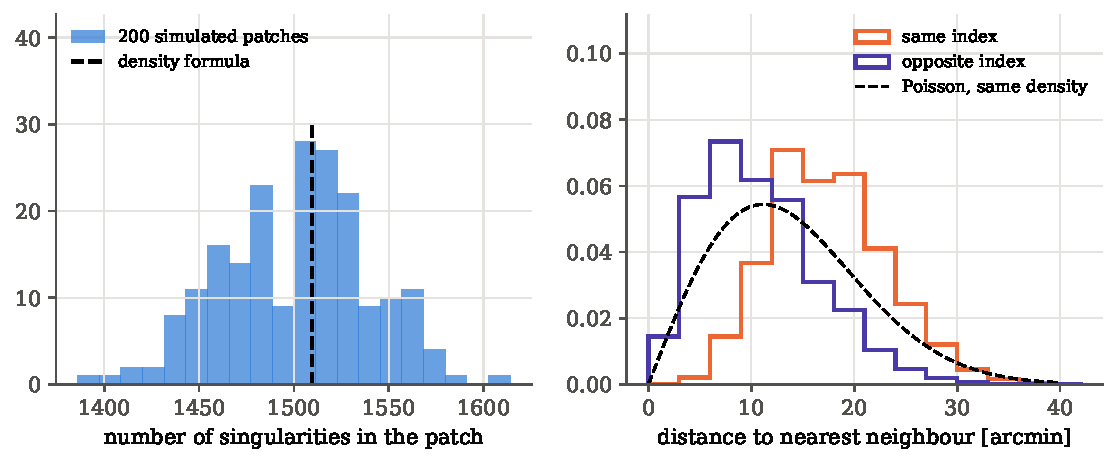
\includegraphics[width=\linewidth]{figures/chT3/pol_stats.pdf}
\caption{Left: number of polarization singularities in \TcNsim\ simulated $10'$-beam patches; the dashed line is the density formula \eqref{T3a:eq:density}. Right: distance from each singularity to its nearest neighbour of the same index and of the opposite index, against the distribution for points scattered at random with the density of one index. Opposite indices sit closer than random points would; equal indices keep apart.}
\label{T3a:fig:polstats}
\end{figure}

\emph{What the arrangement shows.} Huterer and Vachaspati measured three things. The net index inside a closed loop of length $L$ fluctuates with a root-mean-square value growing as $L^{\beta}$ with $\beta\approx0.5$ (between $0.54$ for $\ell_{\max}=100$ and $0.45$ for $500$): the index enclosed is a sum of roughly $L/\xi$ independent contributions from the stretches of the loop, one per correlation length $\xi$, and a sum of that many random terms grows as their square root \cite{VachaspatiLue2003}. Singularities of the same index repel and those of opposite index attract: for $\ell_{\max}=100$ the mean distance to the nearest neighbour of the same index is $3.24^\circ$ and of the opposite index $2.69^\circ$. Beyond about $10^\circ$ the singularities are uncorrelated. The right panel of \cref{T3a:fig:polstats} shows the same attraction and repulsion at $10'$ resolution: mean nearest-neighbour distances of $\TcSame'$ for the same index and $\TcOpp'$ for the opposite one, against $\TcPoisson'$ for random points. Physically, a $+\frac12$ and a $-\frac12$ are the two ends of a short region where the field passes close to zero; they are born together.

Huterer and Vachaspati also found these statistics remarkably robust. Tensor modes, strongly tilted spectra and even strongly non-Gaussian, exponentially distributed $E$ and $B$ coefficients left the scaling exponent, the correlation function and the nearest-neighbour distances unchanged; only skies with grossly broken isotropy moved them. That robustness cuts both ways: the singularity distribution is a poor probe of primordial non-Gaussianity, but any departure from it in real data would point to something that happened to the photons after last scattering, and lensing is the obvious candidate \cite{HutererVachaspati2005}. \Cref{T3a:sec:lensing} shows what lensing actually does.
\section{Lensing moves the pattern but keeps its topology}
\label{T3a:sec:lensing}

Between last scattering and us, every CMB photon passes a few dozen potential wells and hills of the large-scale structure, each of which bends its path by about $10^{-4}$ radians. The bends add up like a random walk to a deflection of about $2.7'$, coherent over a couple of degrees, because the potentials that matter are a few hundred megaparsecs across \cite{LewisChallinor2006} (their \S1.2). The image of the last-scattering surface is therefore not blurred but remapped: each patch is shifted, slightly stretched and slightly sheared. A degree-sized hot spot appears a few per cent larger or smaller than it was. For the shapes of the previous sections this is a nuisance. The question is which of them it can change.

\paragraph{The question.} If the observed sky is the unlensed sky seen through a smooth, slightly distorted window, which morphological numbers come through unchanged, and what could change them anyway?

\subsection{The remapping, for temperature and for polarization}
\label{T3a:sec:remap}

For the temperature the remapping is the one already used in \cref{T3a:sec:lens-mf}: the lensed field in direction $\hat{\bm n}$ is the unlensed field at the displaced point, $\tilde T(\hat{\bm n})=T(\hat{\bm n}+\bm\alpha)$, where the deflection is the gradient of a lensing potential, $\bm\alpha=\nabla\psi$ \cite{ChallinorChon2002} (their eq.~1). On the sphere ``the displaced point'' means: walk a distance $|\bm\alpha|$ along the great circle that leaves $\hat{\bm n}$ in the direction of $\bm\alpha$.

For polarization there is one more step, and it is the point of \cite{ChallinorChon2002}. The Stokes parameters are components of the matrix \eqref{T3a:eq:Pmatrix} in a pair of axes at each point, usually the local north and east directions. Copying the numbers $Q$ and $U$ from the displaced point to $\hat{\bm n}$ would compare components in two different sets of axes, and on a curved sky those axes are rotated relative to each other by an angle that depends on the coordinates. The physical statement is that the polarization \emph{matrix} at the displaced point is carried back to $\hat{\bm n}$ by parallel transport along the great circle, and only then read in the local axes (their eq.~4). The naive copy differs from the transported one by a factor $e^{-2i\chi}$ in $Q+iU$, with $\chi$ a rotation angle of the order of the deflection times a coordinate factor that grows towards the poles (their eqs.~7--8); in the flat-sky limit it vanishes, and in any case the residual rotation of the polarization basis is of order an arcminute and negligible \cite{LewisChallinor2006} (their \S3). The upshot for us is simple: the lensed polarization at $\hat{\bm n}$ is the unlensed polarization at $\hat{\bm n}+\bm\alpha$, the same headless stick carried along.

\subsection{Why the topology survives}
\label{T3a:sec:protect}

\emph{The excursion sets.} The lensed hot region is $\{\hat{\bm n}:T(\hat{\bm n}+\bm\alpha)>\nu\sigma_0\}$. Call the remapping $f(\hat{\bm n})=\hat{\bm n}+\bm\alpha(\hat{\bm n})$. The lensed excursion set is exactly the set of points that $f$ sends into the unlensed excursion set, $\tilde Q_\nu=f^{-1}(Q_\nu)$, with the same threshold, because lensing does not change $\sigma_0$ (\cref{T3a:sec:lens-mf}). If $f$ is smooth and has a smooth inverse, it neither tears regions apart nor glues them together, so $\tilde Q_\nu$ has as many pieces and as many holes as $Q_\nu$. The Euler characteristic at every threshold is unchanged, realisation by realisation. The area and the boundary length are not protected in the same way: they change wherever the image is magnified or sheared, although on the full sky the first-order changes average out because the convergence integrates to zero.

\emph{The singularities.} A lensed singularity sits wherever the unlensed polarization at $f(\hat{\bm n})$ vanishes, so the lensed zeros are the images under $f^{-1}$ of the unlensed ones, one for one. Their indices are unchanged too. A small loop around a lensed zero is mapped by $f$ to a small loop around its parent, and the stick along one loop is the stick along the other; if $f$ keeps the orientation of the sky, the two loops are traversed in the same sense and the number of half-turns is the same. In general a continuous change can only move a singularity, or create or destroy a $+\frac12$ and $-\frac12$ together, since the total index inside any fixed large loop is an integer multiple of $\frac12$ that cannot jump \cite{VachaspatiLue2003}.

\emph{When is the remapping invertible?} Locally, $f$ stretches a small patch by the magnification matrix $\mathsf A=\Id+\partial\bm\alpha$, with entries $\delta_{ij}+\partial_i\alpha_j$ \cite{LewisChallinor2006} (their eq.~1.4). As long as $\det\mathsf A>0$ everywhere, $f$ is a local diffeomorphism that keeps orientation; it fails only where $\det\mathsf A$ passes through zero, on the caustics of strong lensing. With a convergence $\kappa=-\frac12\nabla\cdot\bm\alpha$ whose rms is below $0.1$ even on arcminute scales, CMB lensing is nowhere near that.

\paragraph{Example: how far from a caustic?} In the \TdNreal\ simulated $10^\circ$ patches of \cref{T3a:sec:lens-code} the deflection has an rms of $\TdDefl'$ (lower than the full-sky $2.7'$, because the patch cannot hold the degree-scale modes that carry most of the deflection, and a uniform shift of the whole patch would not matter anyway), the convergence has an rms of $\TdKappa$, and the smallest value of $\det\mathsf A$ anywhere in any patch is $\TdDetMin$. It never comes close to zero.

\subsection{What breaks the protection}
\label{T3a:sec:break}

The protection is exact for the remapping alone. Each of the following steps falls outside it.
\begin{itemize}[itemsep=1pt,leftmargin=1.2em]
  \item \emph{Anything applied after lensing.} The telescope beam convolves the \emph{lensed} sky. Smoothing then lensing is a pure remapping; lensing then smoothing is not, because lensing has already moved power to small scales that the beam partly removes. Two singularities of opposite index closer than the beam can be merged and annihilate; a thin hot bridge can be smoothed away. Instrumental noise, added last, creates and destroys features at the noise scale.
  \item \emph{A finite patch, and local densities.} On a patch with an edge, features cross the edge as they move. Magnification also changes the number of features per unit \emph{observed} area, even though the total is fixed, which is how lensing could leave the small-scale imprint on the singularity distribution that \cite{HutererVachaspati2005} anticipated.
  \item \emph{Splitting into $E$ and $B$.} Lensing turns part of the $E$ pattern into $B$. The singularities of the full $(Q,U)$ field are protected; those of an $E$-only or $B$-only map, built non-locally from it, are not.
  \item \emph{The Gaussian formula itself.} The lensed $\Cell$ has a larger $\tilde\sigma_1$, so plugging it into \eqref{T3a:eq:v1},~\eqref{T3a:eq:v2} predicts more islands. The prediction is wrong for the remapped sky, which is no longer Gaussian: its islands are the old ones, deformed.
\end{itemize}

\subsection{Testing it: lensing simulated patches}
\label{T3a:sec:lens-code}

\pyname{04_lensing_remap.py} draws \TdNreal\ unlensed $10^\circ\times10^\circ$ patches of $T$, $Q$ and $U$ (pixels of $\TdPixArcmin'$) from CAMB's unlensed spectra, a lensing potential $\psi$ from its spectrum $C_\ell^{\psi\psi}$ (CAMB's $C_\ell^{\phi\phi}$), and the deflection $\bm\alpha=\nabla\psi$; the lensed maps are the unlensed ones evaluated at $\bm x+\bm\alpha(\bm x)$ by cubic-spline interpolation. Case~A smooths with a $\TdFwhm'$ beam and then lenses: a pure remapping of a smooth sky. Case~B lenses the raw sky and then applies the beam, which is the order in which a real telescope sees it. For every lensed singularity in case~A, the code follows the deflection back to $\bm x+\bm\alpha(\bm x)$ and asks whether an unlensed singularity of the same index is there.

\begin{figure}[htbp]
\centering
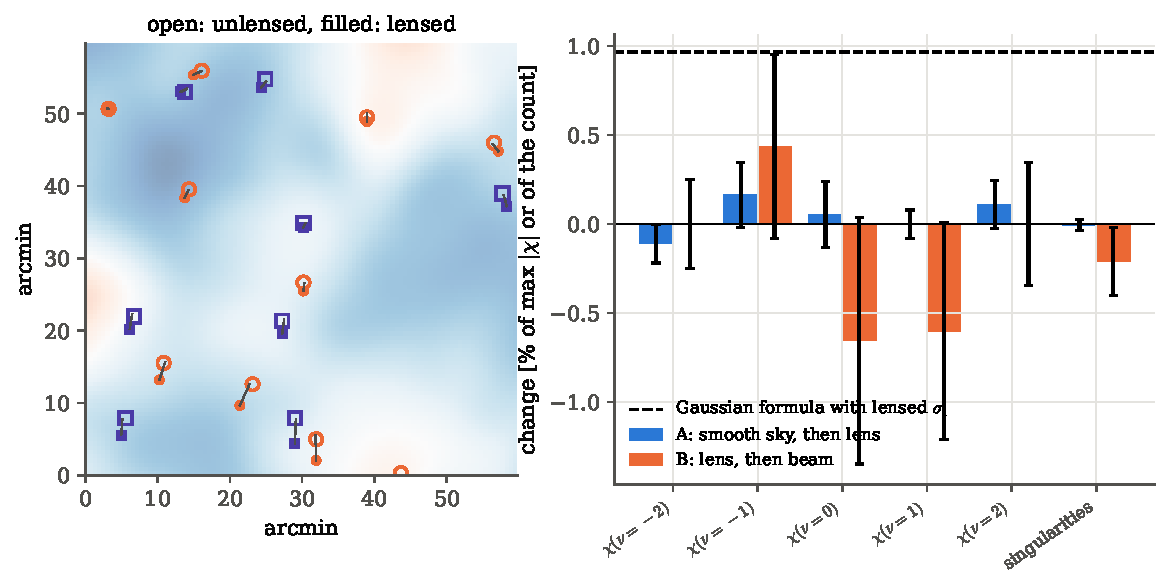
\includegraphics[width=\linewidth]{figures/chT3/lensing_remap.pdf}
\caption{Left: a $1^\circ\times1^\circ$ corner of one patch; open markers are unlensed singularities, filled markers the lensed ones (circles $+\frac12$, squares $-\frac12$), and each grey line joins a lensed singularity to the point its deflection traces back to. Every one lands on a parent of the same index, an arcminute or two away. Right: change of the Euler characteristic at five thresholds and of the singularity count. Case~A (pure remapping) changes nothing beyond pixel-level effects; case~B (beam after lensing) changes them by less than one per cent. Error bars: the patch-to-patch scatter of each change divided by $\sqrt{\TdNreal}$. The dashed line is what the Gaussian formula with the lensed $\sigma_1$ would predict for the Euler characteristic.}
\label{T3a:fig:lensing}
\end{figure}

\Cref{T3a:fig:lensing} shows the outcome. In case~A, \TdMatchPct\% of the lensed singularities (never fewer than \TdMatchMinPct\% in any patch) sit within a pixel and a half of the point the deflection points back to, on a parent of the same index; the rest are pixel-scale ambiguities in where a zero sits inside its $2\times2$ block. The Euler characteristic at every threshold and the singularity count change by at most \TdRelAMaxPct\% of their size, which is the accuracy of counting on a grid. In case~B the singularity count changes by $\TdRelBSingPct\pm\TdRelBSingErrPct\%$ and the Euler characteristic by up to $\TdRelBChiMaxPct\pm\TdRelBChiErrPct\%$ of its peak, where each error is the patch-to-patch scatter of the change divided by $\sqrt{\TdNreal}$. (In case~A the same errors are at most \TdRelAErrMaxPct\%.) Lensing followed by the beam is no longer a pure remapping, so nothing protects the counts. But at a $5'$ resolution the change is small: a few tenths of a per cent, no more than two or three times its error, so $\TdNreal$ patches cannot pin it down. The Gaussian formula with the lensed gradient variance predicts a change of $+\TdGaussPredPct\%$, which these patches can neither confirm nor rule out; and the formula has no right to be used here anyway, because the lensed sky is not a new Gaussian sky.

\paragraph{What this bought us.} For the analysis of real maps the lesson is practical. A topological count (the Euler characteristic, the number of singularities and their indices) is insensitive to lensing to the extent that lensing acts as a remapping, and the residual comes from the instrument's smoothing and noise, which simulations of the instrument capture. The nuisance operator $\mathcal N$ of \cref{ch:12} here is ``lens, then smooth, then add noise''; the first factor is harmless for topology, the last two are not, and that is where the Monte Carlo of \cref{ch:12} has to be careful. The full research version would lens full-sky HEALPix maps at $N_{\rm side}\geq2048$ with the curved-sky remapping and parallel transport of \cite{ChallinorChon2002}, include noise, and use thousands of realisations; the flat $10^\circ$ patches here miss the degree-scale deflection modes, which only shift a patch as a whole, and probe the effect at a single $5'$ resolution.
\section{What \textit{Planck} found}
\label{T3a:sec:planck}

By 2018 the \textit{Planck} temperature maps were limited by cosmic variance over most of the sky and most angular scales: a better instrument would see the same sky. The final release asked, in two papers, the question that the shapes of the previous sections make sharp. Is the CMB a Gaussian, statistically isotropic field, as the simplest inflationary models predict \cite{Planck2018VII}? And if a primordial three-point signal is there, how large can $f_{\rm NL}$ be \cite{Planck2018IX}?

\paragraph{The question.} Measured against simulations of the full \textit{Planck} pipeline, do the shapes of the real maps look like the shapes of Gaussian, isotropic skies? If not, where do they differ, and how surprised should we be?

\subsection{The Minkowski-functional test}
\label{T3a:sec:planck-mf}

\textit{Planck} computes the three functionals of \cref{T3a:sec:mf-def} on masked maps at resolutions from $N_{\rm side}=16$ to $2048$: the area fraction as a pixel count, the boundary length from the contour lengths of all hot and cold spots, and the Euler characteristic as $(N_{\rm hot}-N_{\rm cold})/(2\pi A_{\rm tot})$, the number of compact hot spots minus compact cold spots per area, which is the count of pieces minus holes in another guise \cite{Planck2018VII} (their eqs.~13--15). Two choices are worth noticing, because \cref{ch:12} has to make them too. First, each functional is divided by its Gaussian amplitude, the factor $A_k$ that carries all the dependence on $\sigma_0$ and $\sigma_1$, so that a Gaussian sky would give exactly $v_k(\nu)=e^{-\nu^2/2}H_{k-1}(\nu)$ (their eqs.~16--19, our \eqref{T3a:eq:v0}--\eqref{T3a:eq:v2} rearranged); the thresholds are in units of the map's own standard deviation, as in the pitfall of \cref{T3a:sec:mf-code}. This removes the large cosmic-variance fluctuation of the overall amplitude and keeps the shape. Second, polarization is tested through maps of the scalar $E$ mode, because the functionals of $Q$ and $U$ depend on the orientation of the axes once a mask breaks the symmetry of the sky.

\begin{figure}[htbp]
\centering
\begin{tikzpicture}[
  box/.style={draw=accent,rounded corners=2pt,fill=ideabg,align=center,font=\small,
              minimum width=2.5cm,minimum height=1.0cm,inner sep=3pt},
  arr/.style={->,thick,accent}]
  \node[box] (map) at (0,0) {\textit{Planck} map\\ (masked, $N_{\rm side}$)};
  \node[box] (y) at (3.4,0) {$\bm y$: 3 functionals\\ $\times$ 12 thresholds};
  \node[box] (sims) at (3.4,-2.1) {999 FFP10 sims:\\ $\bar{\bm y}$, $\mathsf C$};
  \node[box] (chi) at (6.9,0) {$\chi^2=(\bm y-\bar{\bm y})\T\mathsf C^{-1}(\bm y-\bar{\bm y})$};
  \node[box] (p) at (6.9,-2.1) {$p=$ fraction of sims\\ with larger $\chi^2$};
  \draw[arr] (map) -- (y);
  \draw[arr] (y) -- (chi);
  \draw[arr] (sims) -- (chi);
  \draw[arr] (chi) -- (p);
\end{tikzpicture}
\caption{The \textit{Planck} Minkowski-functional test. The data vector stacks the three normalised functionals at twelve thresholds between $-3\sigma_0$ and $3\sigma_0$. Its mean and covariance come from end-to-end simulations of Gaussian, isotropic skies processed exactly like the data, and the simulations also supply the distribution of $\chi^2$ under that hypothesis.}
\label{T3a:fig:planck-mf}
\end{figure}

The data vector $\bm y$ stacks $v_0,v_1,v_2$ at twelve thresholds from $-3$ to $3$: 36 numbers per map (\cref{T3a:fig:planck-mf}). Its mean $\bar{\bm y}$ and covariance $\mathsf C$ are estimated from 999 FFP10 simulations, which contain the lensed Gaussian CMB, the instrument's noise, beams and scanning, and the component-separation pipeline. The statistic is $\chi^2=(\bm y-\bar{\bm y})\T\mathsf C^{-1}(\bm y-\bar{\bm y})$ (their eqs.~20--22), and the reported number is the fraction of simulations with a larger $\chi^2$ than the data. This is a hypothesis test in exactly the sense of \cref{ch:04}: the null hypothesis is the one whose sampling distribution we can generate, and the question is whether a $\chi^2$ as large as the observed one, or larger, would be unremarkable if it were true.

\paragraph{Example: the scale of a $\chi^2$ with 36 components.} If $\bm y$ were exactly Gaussian with the estimated mean and covariance, $\chi^2$ would follow a $\chi^2$ distribution with 36 degrees of freedom: mean 36, standard deviation $\sqrt{2\times36}\approx8.5$. A value of 53 would then sit at the 97th percentile. \textit{Planck} does not rely on that shortcut: the simulations give the distribution directly, which also absorbs the noise in $\mathsf C$ estimated from a finite number of simulations (\cref{ch:12}).

\emph{The result.} For temperature, across four component-separation methods and eight resolutions, the probabilities of a larger $\chi^2$ range from about $24\%$ to $99.8\%$: no map is unusual (their Table~5). For $E$-mode polarization most values are similarly unremarkable; a few low ones (down to $1\%$ for one method at $N_{\rm side}=16$) appear for one method and not for the others, which points to residual systematics and noise in the polarization data rather than to the sky. Measured scale by scale, on needlet-filtered maps, the temperature functionals on the largest scales ($\ell\lesssim32$) give probabilities of a few per cent (their Table~6), a mild echo of the large-angle anomalies below. Together with one-point moments, $N$-point correlation functions, peak statistics and the stacking of hot and cold spots, the verdict is: no significant departure from Gaussianity on intermediate and small scales \cite{Planck2018VII}.

\subsection{$f_{\rm NL}$ from the bispectrum}
\label{T3a:sec:planck-fnl}

For a specific three-point shape the bispectrum is the optimal statistic, and \textit{Planck} uses it for the local model \eqref{T3a:eq:local} and for two shapes typical of single-field models with unusual kinetic terms, the equilateral and orthogonal templates. The temperature-plus-$E$ results, after subtracting the expected lensing contribution, are \cite{Planck2018IX}
\begin{equation}
  f_{\rm NL}^{\rm local}=-0.9\pm5.1,\qquad
  f_{\rm NL}^{\rm equil}=-26\pm47,\qquad
  f_{\rm NL}^{\rm ortho}=-38\pm24\qquad(68\%) .
  \label{T3a:eq:fnl}
\end{equation}

\begin{figure}[htbp]
\centering
\begin{tikzpicture}
\begin{axis}[width=9.5cm,height=4.6cm,xmin=-3,xmax=3,ymin=0.5,ymax=5.5,
  xlabel={$f_{\rm NL}/\sigma(f_{\rm NL})$},ytick={1,2,3,4,5},
  yticklabels={{ortho, $T{+}E$},{equil, $T{+}E$},{local, $T{+}E$},{local, $T$, lensing subtracted},{local, $T$, lensing ignored}},
  tick label style={font=\scriptsize},label style={font=\small},axis lines=left,
  extra x ticks={0},extra x tick style={grid=major}]
  \fill[black!6] (axis cs:-2,0.5) rectangle (axis cs:2,5.5);
  \addplot[only marks,mark=*,formblue,error bars/.cd,x dir=both,x explicit]
    coordinates {(-1.583,1) +- (1,0) (-0.553,2) +- (1,0) (-0.176,3) +- (1,0) (-0.089,4) +- (1,0)};
  \addplot[only marks,mark=*,bdryred,error bars/.cd,x dir=both,x explicit]
    coordinates {(1.196,5) +- (1,0)};
\end{axis}
\end{tikzpicture}
\caption{\textit{Planck} 2018 $f_{\rm NL}$ estimates in units of their own standard deviations, with $\pm1\sigma$ bars; the shaded band is $\pm2\sigma$. All are consistent with zero. The red point is the temperature-only local estimate before the lensing contribution is subtracted: lensing alone moves it by more than one standard deviation.}
\label{T3a:fig:fnl}
\end{figure}

\paragraph{Example: what $\pm5.1$ means for the map.} By the Sachs--Wolfe estimate of \cref{T3a:sec:ng-code}, $f_{\rm NL}=5$ skews the large-angle temperature by $|6a|\approx2\times10^{-3}$. The bispectrum detects a three-point signal of this size because it adds up the contributions of millions of triangles of multipoles, each weighted by how well it matches the template; the three Minkowski functionals compress the same map into 36 numbers that are not tuned to any one shape. That is the division of labour: the bispectrum to measure a known shape, the functionals to look for anything unexpected.

\subsection{The anomalies}
\label{T3a:sec:anomalies}

A handful of large-angle features, first seen by WMAP, are confirmed in the \textit{Planck} temperature maps \cite{Planck2018VII} (their \S\S6--7). The variance of the map at low resolution is low: about $1\%$ of the simulations have a variance as small. The angular correlation function $C(\theta)$ is almost zero beyond $60^\circ$: the statistic $S_{1/2}=\int_{-1}^{1/2}[C(\theta)]^2\,\dd\cos\theta$ is smaller in the data than in all but about $1\%$ of the simulations, and partly because the quadrupole is low (removing it lowers the significance from about $99\%$ to $86\%$ of simulations having a larger value). One half of the sky has more power than the other, a dipolar modulation of the fluctuation amplitude. Odd multipoles carry more power than even ones at the lowest $\ell$, a preference for odd point-parity. And there is the Cold Spot, an unusually deep and wide cold region in the southern hemisphere.

Each of these is a deviation at roughly the $2$--$3\sigma$ level, and each was noticed \emph{before} a statistic was designed to measure it. That makes the quoted significances hard to interpret: among the many statistics one could have computed, some are bound to look unusual by chance (the look-elsewhere effect). Since the temperature on these scales is cosmic-variance limited, more temperature data cannot settle it. Polarization can, because it is generated by different modes. The 2018 polarization maps show no corresponding anomaly (no lack of large-angle correlation, no hemispherical asymmetry, no point-parity violation, no polarization signature of the Cold Spot), but their signal-to-noise on these scales is low, and the absence is not yet strong evidence either way \cite{Planck2018VII}.

\begin{inpractice}[verification and research with the same machinery]
The Gaussian checks of \cref{T3a:sec:mf-code,T3a:sec:density} \emph{verify} known formulas: the simulations had to reproduce \eqref{T3a:eq:v1},~\eqref{T3a:eq:v2} and \eqref{T3a:eq:density}, and they did. In the \textit{Planck} test the same machinery is the \emph{research instrument}: for a masked sky with anisotropic noise, component-separation residuals and lensing, no formula gives the mean, the covariance or the $\chi^2$ distribution of the functionals, and a thousand end-to-end simulations are the only way to get them. \Cref{ch:12} builds that test on simulated skies; \cref{ch:13} applies the summary statistics to real \textit{Planck} maps.
\end{inpractice}
\section{The topology of the cosmic web}
\label{T3a:sec:web}

The same questions can be asked one dimension up. Galaxy surveys and simulations show the matter of the late universe arranged in a web: dense clusters at the nodes, filaments joining them, thin walls, and large empty voids. In 1986, before the web had a name, Hamilton, Gott and Weinberg asked whether its connectivity looked like that of a Gaussian field: were the dense regions isolated clumps in an empty background (a ``meatball'' topology), isolated voids in a dense background (``Swiss cheese''), or two interpenetrating networks, like a sponge in which both the material and the holes are connected \cite{HamiltonGottWeinberg1986}?

\paragraph{The question.} If we take the density contrast $\delta$ of a three-dimensional field, smoothed on some scale, and keep the region with $\delta>\nu\sigma$, how connected is it at each $\nu$, and does a Gaussian field predict a sponge at the median density?

\subsection{The genus of a Gaussian field}
\label{T3a:sec:genus}

In three dimensions the boundary of the excursion set is a surface, and its connectivity is measured by its \newterm{genus}: roughly, the number of tunnels through the set minus the number of separate pieces of the surface. A doughnut contributes $+1$ more than a ball. Per unit volume the convenient definition is $g=-\chi/V$, with $\chi$ the Euler characteristic of the set itself \cite{Pranav2017}: every tunnel adds $+1$ to $g$, while every isolated clump and every isolated void adds $-1$. For a Gaussian field the expectation is \cite{HamiltonGottWeinberg1986,Matsubara2003}
\begin{equation}
  g(\nu)=\frac{1}{4\pi^2}\Big(\frac{\langle k^2\rangle}{3}\Big)^{3/2}(1-\nu^2)\,e^{-\nu^2/2},
  \qquad \langle k^2\rangle=\frac{\langle|\nabla\delta|^2\rangle}{\langle\delta^2\rangle} ,
  \label{T3a:eq:genus3d}
\end{equation}
the three-dimensional counterpart of \eqref{T3a:eq:v1},~\eqref{T3a:eq:v2}: again the spectrum enters only through the ratio of the gradient variance to the field variance, and the shape in $\nu$ is a Hermite polynomial times the Gaussian, now $-H_2(\nu)=1-\nu^2$. Read it from the middle outwards. Near $\nu=0$ the genus is positive: many tunnels, a sponge. For $|\nu|>1$ it is negative: at high thresholds isolated clusters (meatballs), at low thresholds isolated voids (Swiss cheese). A Gaussian field is symmetric between the two, so the curve is even in $\nu$. Gravitational evolution breaks that symmetry, shifting the curve towards a meatball topology, and measuring that shift, at fixed volume fraction as in \cref{T3a:sec:relabel}, is the classic use of the genus statistic \cite{Matsubara2003}.

\paragraph{Example: a simulated box.} \pyname{05_web_genus.py} draws \TeNs\ periodic boxes of $\TeN^3$ cells of side $\TeCell\,h^{-1}$Mpc, with a power spectrum $P(k)\propto k^{-1.5}$ smoothed on $\TeR\,h^{-1}$Mpc, and counts the Euler characteristic of the excursion sets as vertices minus edges plus faces minus cubes of the union of voxels, the three-dimensional version of the counter of \cref{T3a:sec:mf-code} (on one box it agrees with scikit-image: \TeEulerOurs\ and \TeEulerSkimage). At the median density a box has a genus of \TeGzeroSim, against \TeGzeroTh\ from \eqref{T3a:eq:genus3d}; over all thresholds the mean of the boxes stays within \TeDevPct\% of the peak of the formula, with a Monte Carlo error of \TeErrPct\% (\cref{T3a:fig:genus}). A Gaussian field is a sponge.

\begin{figure}[htbp]
\centering
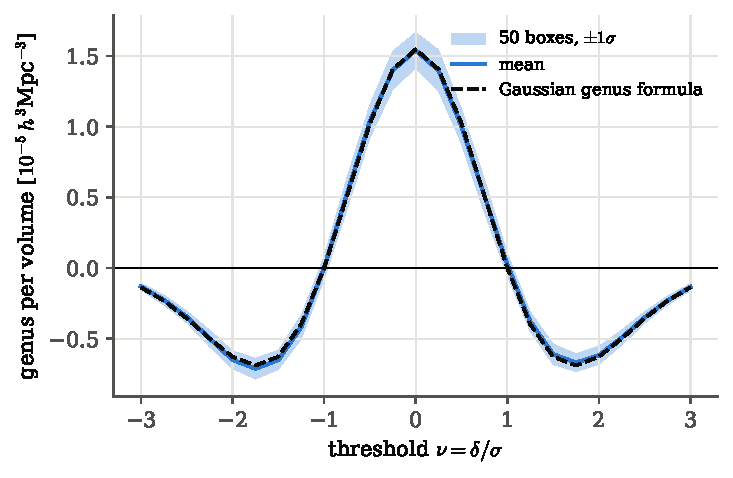
\includegraphics[width=0.62\linewidth]{figures/chT3/web_genus.pdf}
\caption{Genus per unit volume of the excursion sets of simulated three-dimensional Gaussian fields against the threshold. Band: box-to-box scatter; solid: mean of \TeNs\ boxes; dashed: the Gaussian formula \eqref{T3a:eq:genus3d}. Positive genus near the median density means many tunnels (a sponge); negative genus at $|\nu|>1$ means isolated clumps or isolated voids.}
\label{T3a:fig:genus}
\end{figure}

\subsection{Betti numbers and persistence}
\label{T3a:sec:betti}

The Euler characteristic is an alternating sum, $\chi=\beta_0-\beta_1+\beta_2$, of three counts, the \newterm{Betti numbers} \cite{Pranav2017}: $\beta_0$ counts separate pieces (clusters), $\beta_1$ independent tunnels or loops (the loops formed by filaments), and $\beta_2$ enclosed cavities (voids sealed inside the set); see the topology notes for why they are well defined. A sum with alternating signs can hide its terms: two isolated clusters and one hollow shell around a void both have $\chi=2$ (\cref{T3a:fig:betti}). Pranav and collaborators showed that the Betti numbers separately, as functions of the threshold, distinguish web-like models that the genus alone does not, and they introduced \emph{persistence}: follow each feature as the threshold is lowered, record the level at which it appears and the level at which it merges or fills in, and plot the pairs \cite{Pranav2017}. A feature that persists over a wide range of thresholds is a robust structure; one that lives only briefly is noise. \Cref{ch:12} builds these tools from scratch.

\begin{figure}[htbp]
\centering
\begin{tikzpicture}
  \begin{scope}
    \fill[formblue!35] (0,0) circle (0.7) (2.1,0) circle (0.7);
    \draw[formblue,thick] (0,0) circle (0.7) (2.1,0) circle (0.7);
    \node[lbl,align=center,anchor=north] at (1.05,-1.2) {two solid clusters\\ $\beta_0=2,\ \beta_1=0,\ \beta_2=0$\\ $\chi=2$};
  \end{scope}
  \begin{scope}[xshift=6cm]
    \fill[formblue!35,even odd rule] (0,0) circle (1.0) (0,0) circle (0.55);
    \draw[formblue,thick] (0,0) circle (1.0) (0,0) circle (0.55);
    \node[lbl,align=center,anchor=north] at (0,-1.2) {one shell around a void\\ $\beta_0=1,\ \beta_1=0,\ \beta_2=1$\\ $\chi=2$};
  \end{scope}
\end{tikzpicture}
\caption{Cross-sections of two three-dimensional sets with the same Euler characteristic. Left: two separate solid balls. Right: a single hollow ball, whose interior cavity is a sealed void. The Euler characteristic cannot tell them apart; the Betti numbers can.}
\label{T3a:fig:betti}
\end{figure}

Three later studies show what this buys in practice. In $\Lambda$CDM simulations, the persistence diagrams of clusters, filament loops and voids have sharp apexes, and the apex for clusters sits at the density at which matter typically detaches from the Hubble expansion and begins to collapse; persistence diagrams track the hierarchical build-up of the web more informatively than the Euler characteristic or the Betti numbers alone \cite{Wilding2021}. In halo catalogues from $N$-body simulations, persistent homology detects a local primordial non-Gaussianity of $f_{\rm NL}^{\rm loc}=10$ at $97.5\%$ confidence in about $85\%$ of $40\,(h^{-1}{\rm Gpc})^3$ volumes, using information at $\sim10\,h^{-1}$Mpc that is complementary to the scale-dependent bias of the power spectrum \cite{Biagetti2021}. And in weak-lensing mass maps, persistent Betti numbers fed to an emulator and an MCMC give constraints on $S_8=\sigma_8\sqrt{\Omega_m/0.3}$ that are $5\%$ tighter than peak counts for a KiDS-like survey and, for a $100\,{\rm deg}^2$ Euclid-like mock, $18\%$ tighter on $S_8$ and $10\%$ on $\Omega_m$ \cite{Heydenreich2021}. In each case the topological summary is an ordinary random observable, with a mean and a covariance taken from simulations and a likelihood built on them, which is the machinery of \cref{ch:12,ch:09,ch:10}.

The full research version of the experiment above would replace the Gaussian boxes by $N$-body simulations or galaxy catalogues of a few $h^{-3}{\rm Gpc}^3$, add redshift-space distortions and a survey mask, and compute Betti curves and persistence diagrams; the $128^3$ Gaussian boxes here only verify the Gaussian baseline that those analyses measure departures from.
\section*{Chapter summary}
\addcontentsline{toc}{section}{Chapter summary}
\label{T3a:sec:summary}

The microwave sky carries information in its pattern, not only in its amplitudes. Its temperature map is cut at thresholds into excursion sets whose area, coastline and connectivity are three numbers per threshold; a Gaussian sky fixes all three through $\sigma_0$ and $\sigma_1$, a pointwise skewness merely relabels the threshold, and what survives at fixed area fraction is non-local physics. Its polarization has half-integer singularities whose number is a moment of the spectrum and whose arrangement is robust. Lensing remaps both patterns smoothly, which leaves their topology intact until the instrument smooths and adds noise. \textit{Planck} found the sky consistent with Gaussianity and isotropy apart from a few large-angle anomalies of debated significance, and $f_{\rm NL}$ consistent with zero. \Cref{T3a:tab:summary} collects the pieces.

\begin{table}[htbp]
\centering
\small
\renewcommand{\arraystretch}{1.15}
\begin{tabularx}{\linewidth}{>{\raggedright\arraybackslash}p{3.1cm}>{\raggedright\arraybackslash}X>{\raggedright\arraybackslash}p{2.5cm}}
\toprule
Concept & Operational meaning & Used in\\
\midrule
excursion set $Q_\nu$ \eqref{T3a:eq:excursion} & pixels with $T>\nu\sigma_0$ & \cref{ch:12}\\
$v_0,v_1,v_2$ (\cref{T3a:sec:mf-def}) & area fraction; $\frac14$ boundary length per area; pieces minus holes per area & \cref{ch:12,ch:13}\\
$\sigma_0,\sigma_1,\theta_c$ \eqref{T3a:eq:sigma0}--\eqref{T3a:eq:thetac} & variance of the map and of its gradient from $\Cell$; their ratio is the correlation angle & \cref{ch:12}\\
Gaussian functionals \eqref{T3a:eq:v0}, \eqref{T3a:eq:v1}, \eqref{T3a:eq:v2} & $\frac12\operatorname{erfc}$, $e^{-\nu^2/2}$, $\nu e^{-\nu^2/2}$ curves; derived in \cref{ch:12} & \cref{ch:12}\\
skewness parameters, Matsubara correction \eqref{T3a:eq:skewpar}--\eqref{T3a:eq:matsubara} & first-order non-Gaussian change of the curves & \cref{ch:12}\\
area threshold $\nu_A$ (\cref{T3a:sec:relabel}) & label sets by area fraction; removes pointwise distortions & \cref{ch:12}\\
local $f_{\rm NL}$ \eqref{T3a:eq:local} & quadratic piece of the potential; $a=-3f_{\rm NL}\sigma_t$ in the Sachs--Wolfe limit & \cref{ch:12,ch:13}\\
polarization index \eqref{T3a:eq:alpha} & half-turns of the stick around a zero of $Q+iU$; $\pm\frac12$ & \cref{ch:12}\\
singularity density \eqref{T3a:eq:density}, \eqref{T3a:eq:Nsky} & $\sigma_1^2/4\pi\sigma_0^2$; full sky $\langle\ell(\ell+1)\rangle_P$ & \cref{ch:12}\\
lensing remapping (\cref{T3a:sec:remap}) & $\tilde X(\hat{\bm n})=X(\hat{\bm n}+\bm\alpha)$, polarization parallel-transported & \cref{ch:12,ch:13}\\
protected / unprotected (\cref{T3a:sec:protect,T3a:sec:break}) & topology kept by an invertible remapping; broken by beam, noise, edges, $E/B$ split & \cref{ch:12}\\
MF $\chi^2$ test (\cref{T3a:sec:planck-mf}) & 36-vector against end-to-end simulations; $p$ from simulations & \cref{ch:04,ch:12,ch:13}\\
\textit{Planck} $f_{\rm NL}$ \eqref{T3a:eq:fnl} & bispectrum constraints; lensing bias & \cref{ch:12,ch:13}\\
genus, Betti numbers (\cref{T3a:sec:genus,T3a:sec:betti}) & $g=-\chi/V$; $\chi=\beta_0-\beta_1+\beta_2$; persistence & \cref{ch:12,ch:11}\\
\bottomrule
\end{tabularx}
\caption{Every concept of the chapter, how to compute or recognise it, and where the book uses it next.}
\label{T3a:tab:summary}
\end{table}

\subsection*{Reading the literature}
\label{T3a:sec:reading}

\begin{itemize}[itemsep=2pt,leftmargin=1.2em]
  \item J.~Schmalzing and K.~M.~G\'orski, Minkowski functionals used in the morphological analysis of CMB anisotropy maps \cite{SchmalzingGorski1998}: the three functionals on the sphere, their Gaussian expectations and pixel estimators.
  \item T.~Matsubara, Statistics of smoothed cosmic fields in perturbation theory \cite{Matsubara2003}: the first non-Gaussian correction to the genus and the Minkowski functionals, and the area-fraction threshold.
  \item J.~M.~Bardeen, J.~R.~Bond, N.~Kaiser and A.~S.~Szalay, The statistics of peaks of Gaussian random fields \cite{BBKS1986}: spectral moments and the geometry of Gaussian fields.
  \item A.~J.~S.~Hamilton, J.~R.~Gott and D.~Weinberg, The topology of the large-scale structure of the universe \cite{HamiltonGottWeinberg1986}: the genus curve and the sponge.
  \item T.~Vachaspati and A.~Lue \cite{VachaspatiLue2003} and D.~Huterer and T.~Vachaspati \cite{HutererVachaspati2005}: polarization singularities, their index, and their distribution in simulated maps.
  \item A.~Challinor and G.~Chon, Geometry of weak lensing of CMB polarization \cite{ChallinorChon2002}, and A.~Lewis and A.~Challinor, Weak gravitational lensing of the CMB \cite{LewisChallinor2006}: the lensing remapping on the sphere.
  \item \textit{Planck} 2018 results VII and IX \cite{Planck2018VII,Planck2018IX}: tests of isotropy and Gaussianity, the anomalies, and $f_{\rm NL}$.
  \item P.~Pranav et al.\ \cite{Pranav2017}, G.~Wilding et al.\ \cite{Wilding2021}, M.~Biagetti, A.~Cole and G.~Shiu \cite{Biagetti2021}, S.~Heydenreich, B.~Br\"uck and J.~Harnois-D\'eraps \cite{Heydenreich2021}: Betti numbers and persistence in the cosmic web, in halo catalogues and in weak lensing.
\end{itemize}

\begin{recap}
\begin{itemize}[itemsep=1pt,leftmargin=1.2em]
  \item The Minkowski functionals of the excursion sets (area fraction, boundary length, Euler characteristic) are the complete set of additive, motion-invariant shape numbers in two dimensions.
  \item For a Gaussian sky: $v_0=\frac12\operatorname{erfc}(\nu/\sqrt2)$ needs no spectrum; $v_1\propto e^{-\nu^2/2}/\theta_c$ and $v_2\propto\nu e^{-\nu^2/2}/\theta_c^2$ need only $\theta_c=\sigma_0/\sigma_1$.
  \item A pointwise increasing distortion only relabels thresholds; at fixed area fraction it vanishes exactly. Local $f_{\rm NL}$ is such a distortion on Sachs--Wolfe scales.
  \item Polarization singularities have index $\pm\frac12$; their density is $\sigma_1^2/4\pi\sigma_0^2$, about $\langle\ell(\ell+1)\rangle_P$ on the full sky; opposite indices attract, equal ones repel.
  \item Lensing is a smooth invertible remapping: it moves singularities and islands but keeps their number and index; the beam and noise applied afterwards break the protection slightly.
  \item \textit{Planck}: Gaussian and isotropic within errors on intermediate and small scales; a few large-angle anomalies at the $2$--$3\sigma$ level; $f_{\rm NL}^{\rm local}=-0.9\pm5.1$.
  \item In three dimensions the genus curve of a Gaussian field is a sponge at the median density; Betti numbers and persistence separate what the genus adds together.
\end{itemize}
\end{recap}
  